%\documentclass[notes,ignorenonframetext,russian,hyperref={pdftex,unicode}]{beamer}  % слайды и текст лекций
%\documentclass[notes=only,ignorenonframetext,russian,hyperref={pdftex,unicode}]{beamer}     % только текст к лекциям
\documentclass[ignorenonframetext,russian,hyperref={pdftex,unicode}]{beamer}        % только слайды
\usepackage[utf8]{inputenc}
\usepackage[T1,T2A]{fontenc}

\usepackage[russian,english]{babel}
\usepackage{beamerthemesplit}
\usepackage{xifthen}
\usepackage{longtable}
\usepackage{multicol}
\usepackage{verbatim}
\usepackage{listings}

%\usepackage{bibentry}
%\nobibliography*
%\let\newblock\relax


\addto\captionsenglish{%
  \renewcommand{\figurename}{Рис.}%
}

\usetheme{boxes}
%\usetheme{CambridgeUS} %%%%%
 %%%%%
%\usetheme{Montpellier}
%\usetheme{Singapore}


%\usecolortheme{crane}
\usecolortheme{dolphin}
%\usecolortheme{whale}


\title{Обзор возможностей QGIS}
%\author{Колесов Д.А.}
%\author{\texorpdfstring{Колесов Д.А.\newline\url{kolesov.dm@gmail.com}}{Колесов Д.А.}}
\institute{NextGIS}
\date{2014}



\begin{document}

\frame{\titlepage}

\begin{frame}[allowframebreaks]
    \frametitle{Содержание}
    %\begin{multicols}{2}
       \tableofcontents
    %\end{multicols}
\end{frame}



\mode<all>

\section{Общие сведения о ГИС. QGIS как пример геоинформационной системы.}
    \subsection{Что такое ГИС.}
    
\begin{frame}
    \frametitle{Что такое ГИС?}
    \begin{description}
        \item[Геоинформационная система; ГИС:] Информационная система,
        оперирующая пространственными данными [ГОСТ Р 52438-2005];

        \item[информационная система:] Система, предназначенная для хранения,
        обработки, поиска, распространения, передачи и
        представления информации [ГОСТ 7.0-99];

        \item[информационная система:] совокупность содержащейся в базах
        данных информации и обеспечивающих ее обработку информационных т
        ехнологий и технических средств [N 149-ФЗ].

    \end{description}

    Геоинформационная система (ГИС) ---
    система сбора, хранения, анализа и графической визуализации
    пространственных (географических) данных и связанной с ними
    информацией о необходимых объектах.

\end{frame}

\begin{frame}
    \frametitle{Что такое ГИС?}
    \begin{figure}[!ht]
        \begin{center}
            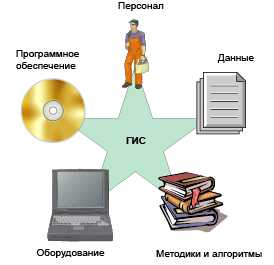
\includegraphics[width=0.4\columnwidth]{./introduction/img/what-is-gis.png}
        \end{center}
    \end{figure}
    Совокупность программно-аппаратных средств, обученного персонала,
    способных создавать, хранить, показывать и анализировать данные о
    расположении и свойствах объектов в пространстве.
\end{frame}
\note{
Сказать, что все части важны. Обратить
внимание, что тут нет ни слова про
карту, потому что ГИС --- это не карта, пусть даже электронная.
ГИС --- это гораздо больше.

Перейти к тому, что ниже мы будем рассматривать не все
компоненты, а только то, что нас интересует больше всего:
\begin{itemize}
    \item Данные;
    \item Методики;
    \item ПО;
\end{itemize}
}


    \subsection{Организация данных в ГИС.}
    

\begin{frame}
    \frametitle{Определение}
    \begin{description}
        \item[Геоданные:] данные о пространственных объектах и явлениях.
        \item[Пространственный объект:] цифровая модель материального или абстрактного объекта реального или виртуального мира включающая его идентификаторы, координатные и атрибутивные данные.
    \end{description}
\end{frame}

\begin{frame}
    \frametitle{Особенности пространственных данных.}
    \begin{itemize}
        \item геопространственные системы координат
        \item высокая информационная насыщенность
        \item объединение геометрической и атрибутивной информации
        \item послойная организация
    \end{itemize}
\end{frame}

\begin{frame}
    \frametitle{Явное нахождение в одной и пространственных систем координат.}
    \begin{multicols}{2}
       \begin{figure}[!ht]
           \begin{center}
               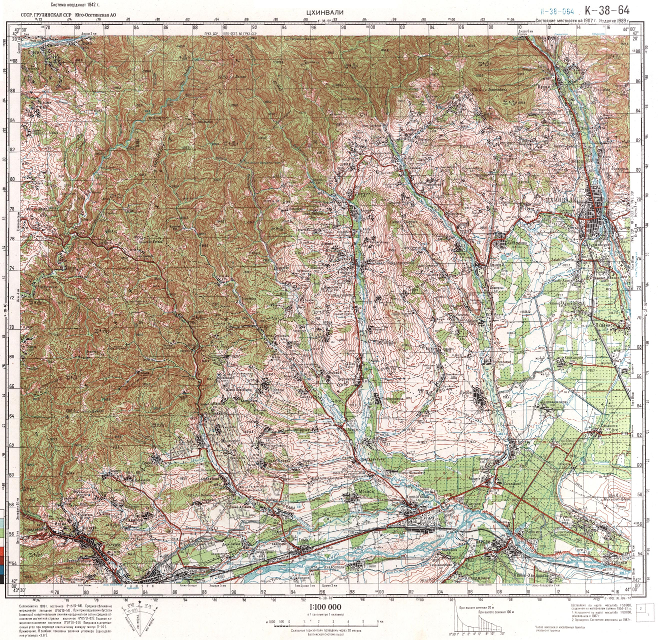
\includegraphics[width=0.8\columnwidth]{./introduction/img/topo_map}
           \end{center}
           \caption{Отсканированное изображение, каждый элемент имеет X,Y,Z}
       \end{figure}

       \begin{figure}[!ht]
           \begin{center}
               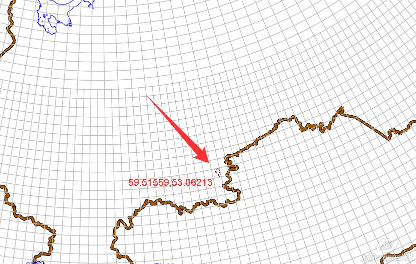
\includegraphics[width=0.95\columnwidth]{./introduction/img/grid_map}
           \end{center}
           \caption{Географически привязанное изображение, каждый элемент имеет широту, долготу, Z}
       \end{figure}
    \end{multicols}
\end{frame}

\begin{frame}
    \frametitle{Высокая информационная насыщенность}
    \begin{description}
        \item[MODIS] Передача 10.6 миллионов бит данных в секунду, т.е. около 53 Тб данных в день.
        \item[OpenStreetMap] (на начало ноября 2014):
            \begin{itemize}
                \item Число пользователей: 1.85 миллиона;
                \item Число узлов: 2597 миллионов;
                \item Число загруженных точек GPS: 4384 миллионов.
            \end{itemize}
    \end{description}
\end{frame}

\begin{frame}
    \frametitle{Послойная организация}
    \begin{figure}[!ht]
        \begin{center}
            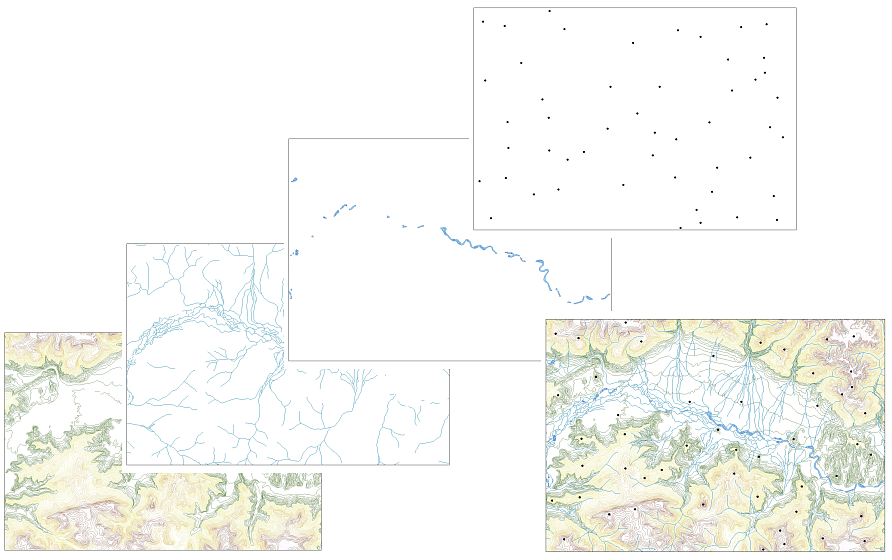
\includegraphics[width=0.9\columnwidth]{./introduction/img/layers_map}
        \end{center}
    \end{figure}
\end{frame}


\begin{frame}
    \frametitle{Объединение геометрической и атрибутивной информации}
    \begin{figure}[!ht]
        \begin{center}
            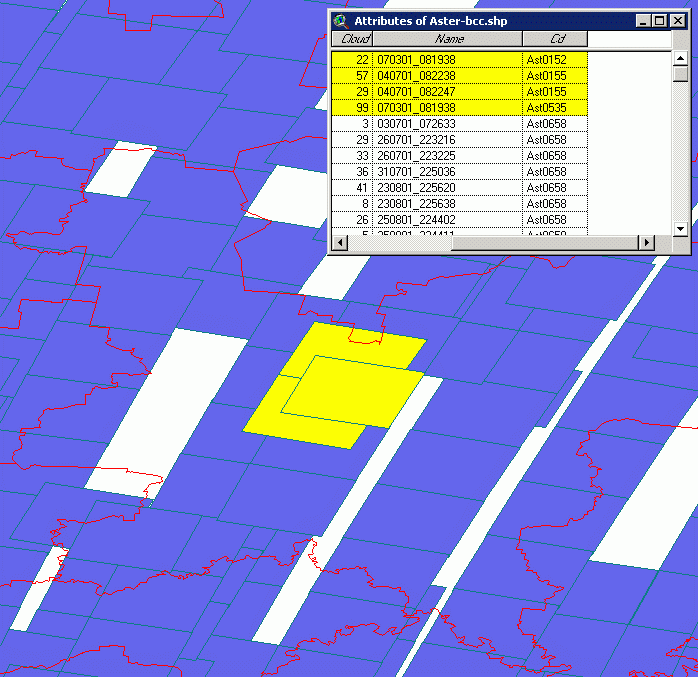
\includegraphics[width=0.55\columnwidth]{./introduction/img/attributes_and_geo}
        \end{center}
    \end{figure}
    Каждый элемент геометрии связан с набором атрибутивных полей (shape --- простая таблица, sqlite/spatialite, PodtgreSQL/PostGIS --- полноценная БД).
\end{frame}


\begin{frame}
    \frametitle{Типы данных}
    Два основных представления данных в ГИС:
    \begin{itemize}
        \item Векторный: обычно используется для представления дискретных объектов, имеющих четкие границы (в масштабе задачи). Например, домов, дорог, озер, \dots
        \item Растровый: часто используется для представления непрерывных объектов и явлений, но может использоваться и для представления дискретных объектов. Основное требование к растровому представлению данных --- размер ячейки должен быть
        значительно меньше, чем размеры объектов.
    \end{itemize}
\end{frame}



    \subsection{Задачи, решаемые с помощью ГИС.}
    

\begin{frame}
    \frametitle{Задачи, решаемые с помощью ГИС}
    \begin{itemize}
        \item Визуализация.
        \item Организация данных.
        \item Картирование природных и антропогенных
            объектов и явлений: идентификация объектов и их состояния, количества, формы, свойств.
        \item Анализ пространственного распределения
            объектов и явлений: плотности, частоты, связность.
        \item Выявление причинно-следственных связей между пространственным
            распределением объектов и явлений и другими данными.
        \item Моделирование и прогнозирование пространственно распределенных процессов.
    \end{itemize}
\end{frame}
\note{
    Перечислить задачи. Сказать, что это лишь примеры,
    между многими задачами нет четкой границы.
    Например, анализ и выявление связей --- перетекающие друг в друга задачи.

    Сказать, что дальше пойдут примеры конкретных
    приложений, которые делались у нас или с нашим участием. Рассказываем про наши, потому, что знаем их в деталях
    и можем рассказать во всех подробностях.
}

\begin{frame}
    \frametitle{Информационная система по объектам животного и растительного мира}
    Информационная система по объектам животного и растительного мира ХМАО (\url{http://ugrabio.ru/}):
    \begin{itemize}
        \item обеспечение удаленного доступа к Базе Данных (далее БД) о распространении биологических видов, в т.ч. видов занесенных в Красную книгу ХМАО;
        \item осуществление сбора информации об объектах
        животного и растительного мира ХМАО от
        респондентов (сотрудников ООПТ, профильных НИИ и университетов) посредством сети Интернет;
        \item обеспечение возможности первичного
        (визуального) анализа распространения биологических таксонов на автоматически генерируемых из БД картах-схемах;
        \item обеспечение возможности использования
        исходных данных БД для различных методов анализа с использованием стороннего программного обеспечение (функция экспорта первичных данных).
    \end{itemize}
\end{frame}
\note{
Показать веб-сайт, рассказать о проекте.
}

\begin{frame}
    \frametitle{ГИС для Красногорска}

\end{frame}

\begin{frame}
    \frametitle{InaSAFE}
    InaSAFE --- свободное программное обеспечение по
    формированию реалистичных сценариев природных
    угроз (стихийных бедствий) для планирования и подготовки ответных мер. Создано на базе QGIS.

    Примеры вопросов, на которые может ответить
    система: если будет наводнение/землятресение/\dots такое же, как в \dots году, то
    \begin{itemize}
        \item Какие дороги будут разрушены/затоплены?
        \item Какие области потребуется эвакуировать?
        \item Сколько понадобится организовать
        эвакуационных лагерей, какое количество еды/воды, медикоментов будет необходимо?
        \item \dots
    \end{itemize}

    Ответы строятся на основе функций, содержащих
    <<стандартные>> операции растрового и векторного анализа.
\end{frame}

\begin{frame}
    \frametitle{MOLUSCE --- анализ динамики состояния территорий}
    \begin{itemize}
        \item Есть территрория и классы землепользования
        (например, лес, городская застройка, сельхозугодья)
        \item Известно, как эта территория изменялась в прошлом.
        \item Построить прогноз будущих изменений.
    \end{itemize}
    Используются методы машинного обучения.
\end{frame}
\note{
Сказать, что это не по-тупому, а там можно создвать
сложные запросы. Например, происходит изчезновение
лесов, один из вариантов сдерживания -- организация
заповедника (другой вариант изменение законодательства на уменьшение рубок).
Вопросы: поможет ли это вообще (может не
антропогенная причина основная)? Где нужно размещать
заповедник, чтобы получить максимальную отдачу
(ограничения: на площадь, запрет на определенные местоположения заповедников).
}

\begin{frame}
    \frametitle{MOLUSCE --- анализ динамики состояния территорий}
    \begin{figure}[!ht]
        \begin{center}
            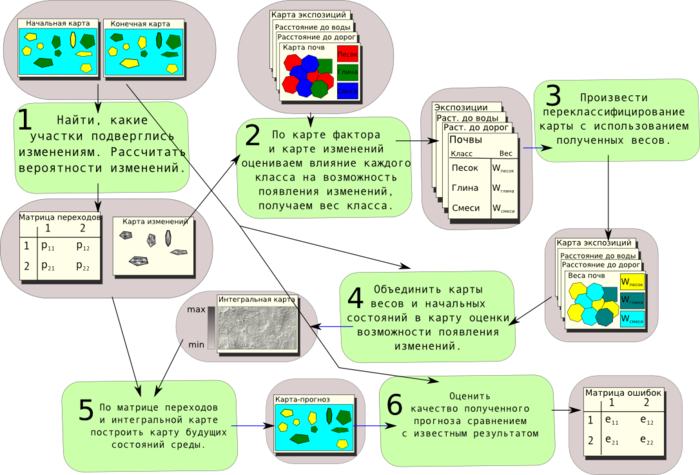
\includegraphics[width=0.9\columnwidth]{./introduction/img/MOLUSCE}
        \end{center}
    \end{figure}
\end{frame}
\note{
Про технологию модуля
}



    %~ \subsection{Классификация ГИС по их функциональности.}
    %~ 




    \subsection{Источники информации по ГИС и пространственным данным.}
    

\begin{frame}[allowframebreaks]
    \frametitle{Источники информации}
    \begin{enumerate}
        \item Сайт специалистов в области         ГИС и ДЗЗ: \url{http://gis-lab.info/}
        \item Сайт открытой ГИС QGIS: \url{http://www.qgis.org/}
        \item QGIS <<русской сборки>> \url{http://nextgis.ru/nextgis-qgis/}
        \item Онлайн-документация QGIS: \url{http://www.qgis.org/ru/site/index.html}
        \item GDAL/OGR - библиотеки обработки         растровых и векторных геоданных:        \url{http://gdal.org/index_ru.html}
        \item PROJ.4: библиотека для        выполнения преобразований систем         координат: \url{http://trac.osgeo.org/proj}
        \item База данных систем координат     European Petroleum Survey Group (EPSG):        \url{http://www.epsg.org}
        \item База с описанием различных         систем координат и проекций:    \url{http://spatialreference.org}
        \item Сайт кураторов открытого ПО    ГИС: \url{http://www.osgeo.org}
        \item Сайт OpenStreetMap:  \url{http://www.openstreetmap.org}
        \item Сайт космической программы Landsat: \url{http://landsat.gsfc.nasa.gov}
        \item Сайт космической программы MODIS: \url{http://modis.gsfc.nasa.gov}
        \item Сайт геологической службы США: \url{http://www.usgs.gov}
    \end{enumerate}
\end{frame}

\begin{frame}
    \frametitle{Обзор обучающей литературы по QGIS}
    \begin{itemize}
        \item Плавное введение в ГИС: \url{http://gis-lab.info/qa/gentle-intro-gis.html}.
        \item Руководство пользователя QGIS:
            \begin{itemize}
                \item актуальная документация по последнюю версию QGIS \url{http://www.qgis.org/ru/docs/user_manual/index.html};
                \item документация в pdf формате \url{http://download.osgeo.org/qgis/doc/manual/}.
            \end{itemize}
    \end{itemize}
\end{frame}




    %~ \subsection{Обзор возможностей QGIS.}
    %~ 
\begin{frame}
    \frametitle{QGIS Desktop}

\end{frame}


\begin{frame}
    \frametitle{QGIS Browser}

\end{frame}

\begin{frame}
    \frametitle{QGIS Server}

\end{frame}

\begin{frame}
    \frametitle{QGIS Web Client}

\end{frame}


\begin{frame}
    \frametitle{QGIS для Android (бета!)}

\end{frame}


\section{Системы координат}
    \subsection{Общие сведения}
    
\begin{frame}
    \frametitle{Системы координат}
    \begin{itemize}
        \item Локальные системы координат
        \item Географические системы координат
        \item Спроецированные (прямоугольные) системы координат
    \end{itemize}
\end{frame}

\begin{frame}
    \frametitle{Как различать по значениям координат}
    \begin{itemize}
        \item Локальные системы координат: от 0,0 до, например, 5000,6000
        \item Географические системы координат: от -180,-90, до 180,90
        \item Спроецированные (прямоугольные) системы координат: от -1000000,1000000 до, например, 1000000, 1000000
    \end{itemize}
\end{frame}


\begin{frame}
    \frametitle{Локальные системы координат}
    \begin{figure}[!ht]
        \begin{center}
            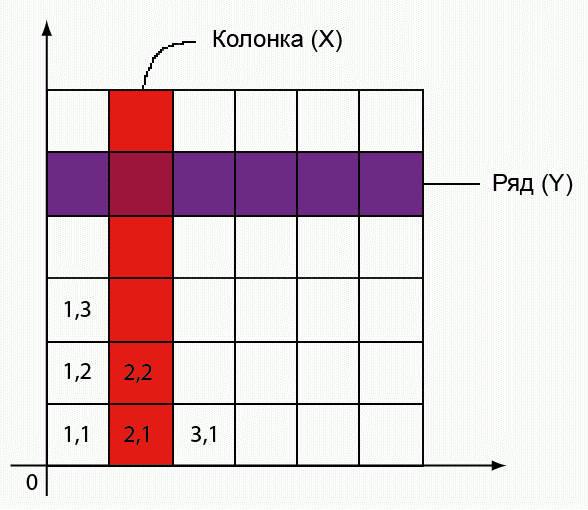
\includegraphics[width=0.6\columnwidth]{./coordinates/img/local_coord}
        \end{center}
    \end{figure}
\end{frame}

\begin{frame}
    \frametitle{Географические координаты}
    \begin{figure}[!ht]
        \begin{center}
            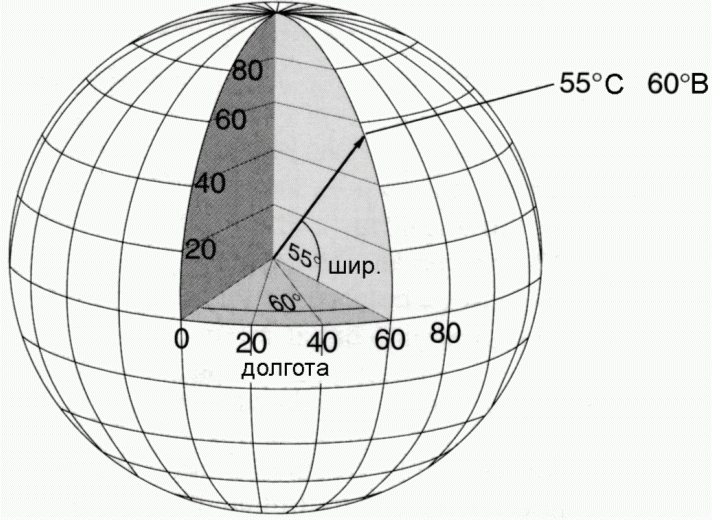
\includegraphics[width=0.6\columnwidth]{./coordinates/img/geo_coord}
        \end{center}
    \end{figure}

    Широта --- угол между  плоскостью экватора и нормалью к поверхности эллипсоида в данной точке (0-90 с.ш. и ю.ш.)

    Долгота --- угол между меридианом данной точки и начальным меридианом (0-180 з.д. и в.д.)
\end{frame}



\begin{frame}
    \frametitle{Геоид}
    \begin{figure}[!ht]
        \begin{center}
            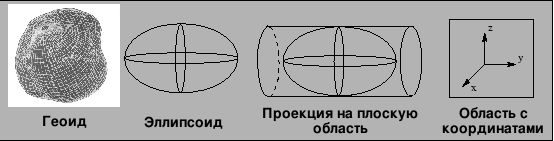
\includegraphics[width=0.7\columnwidth]{./coordinates/img/geoid.png}
        \end{center}
        \caption{Понятие геоида, элипсоида и проекции}
    \end{figure}
    \begin{description}
        \item[Геоид] Форму Земли, особенно с учетом рельефа, можно описать с помощью геоида. Эта фигура является результатом сложных физических расчётов гравитационного поля Земли. Из-за неоднородного распределения массы поле оказывается разным в разных регионах, что приводит к деформации сферы. Таким образом, геоид представляет гравитационое поле Земли.
    \end{description}
    Ввиду математической сложности геоида, в качестве приближения формы Земли в географических информационных системах используется сфера или эллипсоид.
\end{frame}

\begin{frame}
    \frametitle{Эллипсоид}
    \begin{figure}[!ht]
        \begin{center}
            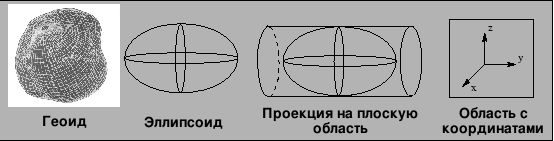
\includegraphics[width=0.8\columnwidth]{./coordinates/img/geoid.png}
        \end{center}
        \caption{Понятие геоида, элипсоида и проекции}
    \end{figure}

    Упрощённое представление формы Земли сферой недостачно точно для создания карт масштаба крупнее 1:2~000~000. Эллипсоиды вращения или сфероиды пытаются воспроизвести сложную форму Земли насколько возможно точно математически. Поэтому расстояние от полюса до центра Земли меньше, чем от экватора.

    Существует ряд моделей эллипсоидов, дающих оптимальные результаты для разных регионов. В общем, для каждого региона можно подобрать эллипсоид, являющийся достаточно точным приближением поверхности Земли в этом регионе.

\end{frame}

\begin{frame}
    \frametitle{Примеры референц-эллипсоидов}
    \begin{table}[h]
    \centering
    \begin{tabular}[c]{p{0.2\linewidth}|p{0.15\linewidth}|p{0.15\linewidth}|p{0.3\linewidth}}
    {Эллипсоид, представ\-ляющий Землю} & Большая полуось (м) & Малая полуось (м) & Область применения\\[2mm]\hline
     WGS 1984 & 6378137 & 6378137 & Северная Америка, весь мир\\
     Эллипсоид Крассовского & 6378245 &6356863 & Российская Федерация, страны бывшего CCCР\\
     & & &
    \end{tabular}\caption{Примеры распространенных эллипсоидов}
    \end{table}
\end{frame}

\begin{frame}
    \frametitle{Датум}
    {\tiny Эллипсоид задаёт абстрактную модель конфигурации земной поверхности. Для того, чтобы можно было отсчитывать координаты точки на поверхности эллипсоида --- нужны оси координат.}

    \begin{description}
        \item[Датум:] набор параметров смещения и поворота референц-эллипсоида для лучшей апроксимации земной поверхности. Также датум задаёт нулевой меридиан, от которого будет идти отсчёт долготы.
    \end{description}
    { \small
   Датумы бывают
   \begin{itemize}
       \item глобальными, т.е. предназначенными для аппроксимации земной поверхности на территории всей планеты. Например, датум WGS84 базирующийся на собственном эллипсоиде.
       \item локальными, т.е. предназначенными для лучшей аппроксимации участка земной поверхности. Пример: <<Пулково 1942>> --- датум, основывающийся на эллипсоиде Крассовского, и предназначенный для лучшей аппроксимации территории Советского Союза.
    \end{itemize}
    }
   {\tiny На базе одного референц-эллипсоида может основываться несколько различных датумов. Так, многие страны восточной Европы имели собственные датумы, основанные на эллипсоиде Крассовского.}
\end{frame}


\begin{frame}
    \frametitle{Переход от одного датума к другому}
    \begin{figure}[!ht]
        \begin{center}
            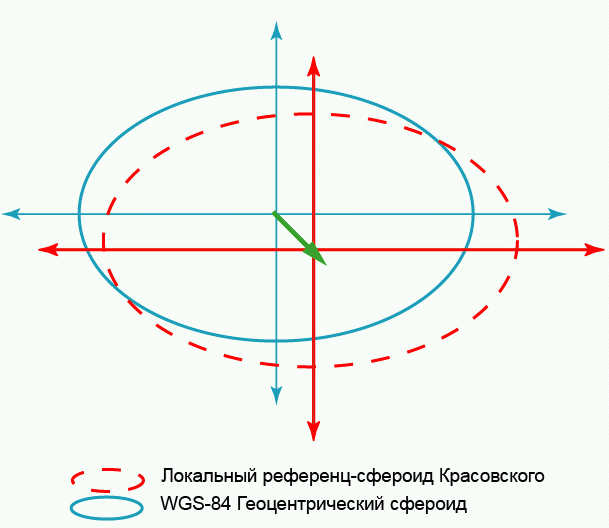
\includegraphics[width=0.6\columnwidth]{./coordinates/img/coord_transition}
        \end{center}
    \end{figure}
\end{frame}


\begin{frame}
    \frametitle{Три семейства картографических проекций\footnote{Материал раздела опирается на "Краткое введение в ГИС" \url{http://gis-lab.info/qa/gentle-intro-gis.html}}}
    \begin{figure}[!ht]
        \begin{center}
            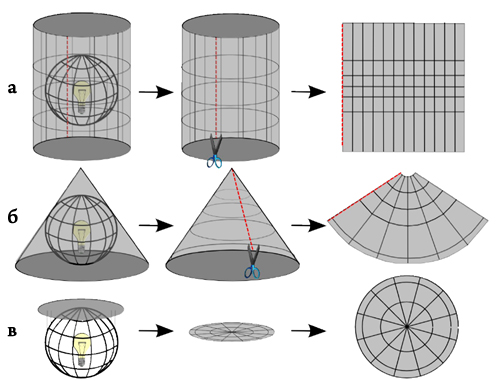
\includegraphics[width=0.75\columnwidth]{./coordinates/img/proj_fam.jpg}
        \end{center}
        \caption{а) цилиндрические, б) конические и в) плоскостные (азимутальные) проекции}
    \end{figure}
\end{frame}

\begin{frame}
    \frametitle{Виды искажений}
    В ходе проецирования любая карта будет иметь искажения
    \begin{itemize}
        \item углов,
        \item расстояний,
        \item площадей.
    \end{itemize}
    возможны искажения одновременно нескольких параметров.

    Поэтому важно подобрать проекцию карты под решаемую задачу.

\end{frame}

\begin{frame}
    %\frametitle{Конформные проекции}
    \begin{description}
        \item[Равноугольная (конформная) проекция:] картографическая проекция, позволяющая передавать на картах углы без искажений и сохранять в каждой точке постоянный масштаб по всем направлениям, хотя в разных местах карты масштаб различен.
    \end{description}
    Используются для навигационных, метеорологических и др. задач, где важно сохранение углов.
    \begin{figure}[!ht]
        \begin{center}
            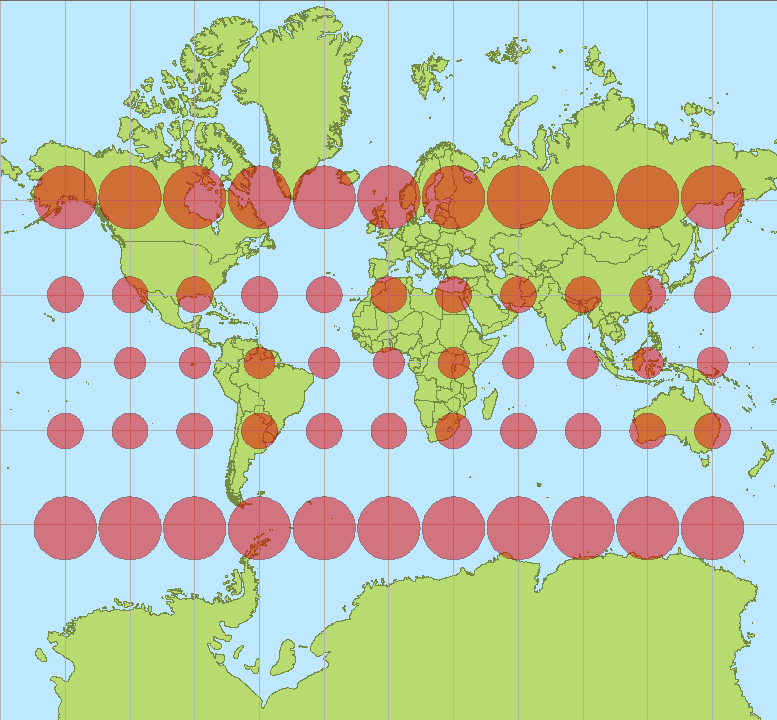
\includegraphics[width=0.5\columnwidth]{./coordinates/img/merkator.png}
        \end{center}
        \caption{Пример --- проекция Меркатора.}
    \end{figure}

\end{frame}

\begin{frame}
    %\frametitle{Равнопромежуточные проекции}
    \begin{description}
        \item[Равнопромежуточная проекция:] картографическая проекция, обладающая свойством сохранения масштаба вдоль определенных линий.
    \end{description}
    Равнопромежуточные проекции обеспечивают правильные расстояния от центра проекции вдоль определенных линий. Эти проекции используются для сейсмического картографирования, а также для задач навигации.
    \begin{figure}[!ht]
        \begin{center}
            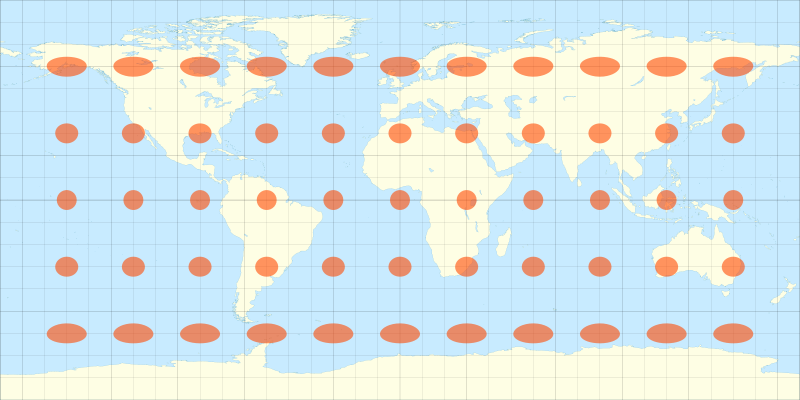
\includegraphics[width=0.8\columnwidth]{./coordinates/img/equidistant.png}
        \end{center}
        \caption{Пример --- простая цилиндрическая проекция (plate carrée)}
    \end{figure}
\end{frame}

\begin{frame}
    %\frametitle{Равновеликие проекции}
    \begin{description}
        \item[Равновеликая проекция:] картографическая проекция, которая не искажает площадей и сохраняет на всей карте единый масштаб площадей
    Площади фигур на карте пропорциональны площадям соответствующих фигур в реальности, но при этом сильны искажения углов и форм.
    \end{description}
    \begin{figure}[!ht]
        \begin{center}
            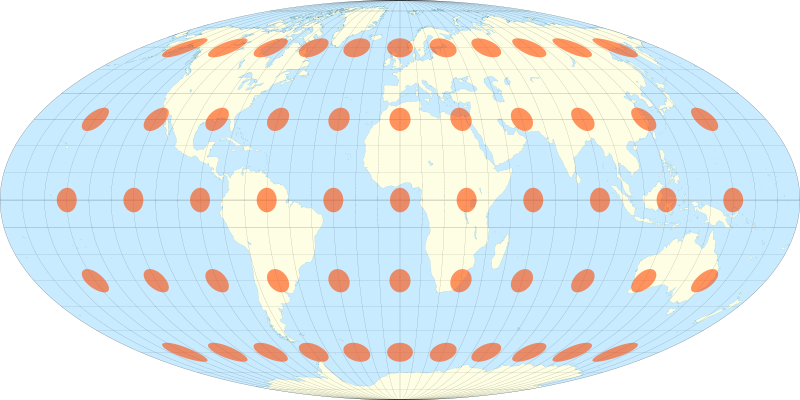
\includegraphics[width=0.85\columnwidth]{./coordinates/img/mollweide.png}
        \end{center}
        \caption{Пример --- равновеликая цилиндрическая проекция Мольвейде }
    \end{figure}

\end{frame}


\begin{frame}
    \frametitle{Системы координат}
    После того, как поверхность земного шара или её часть спроецирована на плоскость, следует задать систему координат, чтобы точно размещать 2-~или 3-мерные участки на карте.

    С помощью систем координат каждое место на Земле может быть описано набором из трех цифр, называемых координатами. Системы координат делят на
    \begin{itemize}
        \item системы географических координат;
        \item системы проекционных координат (также называются картезианскими, или прямоугольными).
    \end{itemize}
\end{frame}

\begin{frame}
    \frametitle{Географические системы координат}

    Географическая система (Longitude-Latitude, lon/lat): Наиболее часто используемая система, использующая долготу, широту и высоту.

    Координаты отсчитываются от нулевого меридиана и экватора. В результате, поверхность земли покрывает сетка из 180 меридианов (долгот) на запад и восток от Гринвича и 180 параллелей (широт) на север и юг от экватора.

    Высота измеряется от центра Земли.

    Единицы системы могут быть выражены в шестидесятеричном (градусы:минуты:секунды, буква, обозначающая направление) или десятичном (+/- градусы с десятичными знаками) исчислении.
\end{frame}


\begin{frame}
    \frametitle{Системы проекционных координат}
    Будут рассмотрены две распространенные системы:
    \begin{itemize}
        \item Система координат (проекция) Гаусса-Крюгера;
        \item Система координат (проекция) UTM (Universal Transverse Mercator)
    \end{itemize}

\end{frame}

\begin{frame}
    \frametitle{Система кординат Гаусса-Крюгера}
    \begin{figure}[!ht]
        \begin{center}
            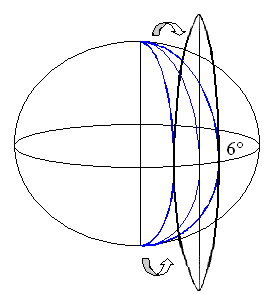
\includegraphics[width=0.4\columnwidth]{./coordinates/img/gauss_kruger1.png}
        \end{center}
        \caption{Схема построения 6-градусных зон}
    \end{figure}
    Вся поверхность Земли делится на 6-градусные (по долготе) зоны (дольки от полюса до полюса), которые каждая отдельно разворачиваются в плоскую поверхность. Всего образуется 60 таких зон, которые нумеруются цифрами от 1 до 60.

\end{frame}

\begin{frame}
    \frametitle{Зоны}
    \begin{figure}[!ht]
        \begin{center}
            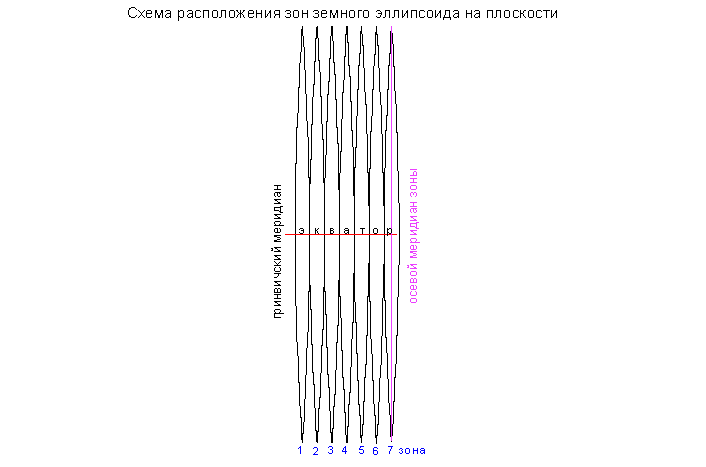
\includegraphics[width=0.6\columnwidth]{./coordinates/img/zonesgk_l.png}
        \end{center}
    \end{figure}
     Зоны нумеруются с запада на восток, начиная с 0: зона 1 простирается с меридиана 0 до меридиана 6, её центральный меридиан 3. Зона 2 --- с 6 до 12, и т.д.

     Цилиндр разворачивают в плоскость и накладывают прямоугольную километровую сетку. За ось OX принимают изображение осевого меридиана зоны (положительное направление --- на север), за ось OY принимают изображение экватора (положительное направление --- на восток).
\end{frame}

\begin{frame}
    \frametitle{Координаты внутри зоны}
    \begin{figure}[!ht]
        \begin{center}
            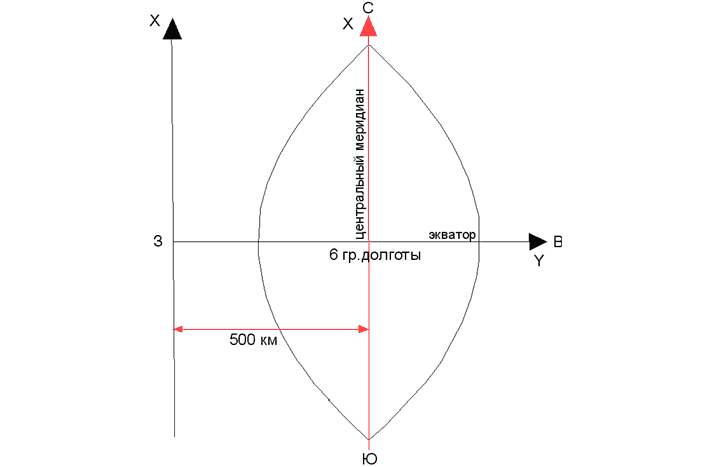
\includegraphics[width=0.35\columnwidth]{./coordinates/img/gauss_kruger2.png}
        \end{center}
    \end{figure}
    В каждой из шестиградусных зон своя система прямоугольных координат. Вертикальные линии сетки параллельны центральному меридиану. Для того, чтобы все прямоугольные координаты были положительны, вводится восточное смещение (false easting), равное 500~000 м, т.е. координата Y на центральном меридиане равна 500~000 м. Для определенности, чтобы только по численному значению координаты Y можно было определить, к какой зоне относятся эти значения, к ним слева приписывается номер зоны.

    Пример: (X=6~177~200; Y=7~420~000) --- 7 зона, на 80 км западнее среднего меридиана зоны 7, на 6~177~200 метров севернее экватора.

\end{frame}

\begin{frame}
    \frametitle{UTM}
    Система координат UTM по построению похожа на систему Гаусса-Крюгера:
    \begin{itemize}
        \item делит Землю на 60 вытянутых в меридиональном направлении зон шириной 6 градусов;
        \item отображающая их по отдельности в равноугольной поперечно-цилиндрической проекции Меркатора.
    \end{itemize}

     Отличия:
     \begin{itemize}
         \item используется масштабный коэффициент, равный 0,9996.% Поэтому эта система координат сохраняет масштабы не на осевом меридиане, а на некотором расстоянии (около 180 км) от него, из-за чего максимальное искажение масштаба в пределах шестиградусной зоны у неё меньше.
         \item нумерация зон: первая зона та, осевой меридиан которой имеет долготу 177 з.д. % Таким образом, например, 7-я зона в системе координат Гаусса—Крюгера по географическому охвату соответствует 37-й зоне UTM.
         \item Ось абсцисс в данной системе координат направлена на восток, а ось ординат --- на север. Во избежание отрицательных значений координат, к значению абсциссы прибавляются 500~000~м, а к значению ординаты в южном полушарии --- 10~000~000~м
     \end{itemize}
\end{frame}

\begin{frame}
    \frametitle{Важно помнить}
    \begin{itemize}
        \item Всегда уточняйте в какой системе координат данные
        \item Убедитесь, что у слоев всегда есть файл описания проекции *.prj
        \item Если это таблица с координатами, уточняйте в каком они формате
    \end{itemize}
\end{frame}



\begin{frame}
    \frametitle{Литература}
    \begin{enumerate}
        \item \url{http://gis-lab.info/docs/grass/tutorial60/04r.html}
        \item \url{http://gis-lab.info/qa/gentle-intro-gis.html}
        \item \url{http://giscraft.ru/info/cs/cs.shtml}
    \end{enumerate}
\end{frame}






    \subsection{PROJ4}
    
\begin{frame}
    \frametitle{PROJ4}
    PROJ4 библиотека для работы с системами координат (используется в GRASS GIS,  MapServer,  PostGIS,  Thuban,  OGDI,  Mapnik,  TopoCad, and  OGRCoordinateTransformation и др.).

    База описаний проекций EPSG (\url{http://www.epsg.org/}) хранит данные в формате PROJ4.
\end{frame}

\begin{frame}[fragile]
    \frametitle{Описание проекций в формате proj4}
    Некоторые параметры:
    \begin{itemize}
        \item \verb!+proj! Название проекции
        \item \verb!+lat_0! Широта начала координат
        \item \verb!+lon_0! Осевой меридиан
        \item \verb!+k! Масштабный коэффициент
        \item \verb!+x! Восточное смещение
        \item \verb!+ellps! Эллипсоид
        \item \verb!+towgs84! Параметры перехода к WGS84
        \item \verb!+units! Единицы измерения
    \end{itemize}


\end{frame}

\begin{frame}[fragile]
    \frametitle{Описание проекций в формате proj4}
    Пример: описание системы координат Гаусса-Крюгера 9-й зоны на эллипсоиде Крассовского:
    \begin{verbatim}
    +proj=tmerc +lat_0=0 +lon_0=51 +k=1
    +x_0=9500000 +y_0=0
    +ellps=krass
    +towgs84=23.92,-141.27,-80.9,-0,0.35,0.82,-0.12
    +units=m
    \end{verbatim}

    Пример: широта/долгота на WGS84:
    \begin{verbatim}
    +proj=longlat +datum=WGS84
    \end{verbatim}
\end{frame}

\begin{frame}[fragile]
    \frametitle{Примеры преобразований}
    Программа cs2cs производит преобразование координат
    заданными в указанных системах координат.
    \begin{verbatim}
    cs2cs +proj=latlong +datum=NAD83
                   +to +proj=utm +zone=10 +datum=NAD27 -r <<EOF
             45d15'33.1"   111.5W
             45d15.551666667N   -111d30
             +45.25919444444    111d30'000w
             EOF
    \end{verbatim}
    Будет произведено преобразование входных координат из широта/долгота на NAD83
     в 10-ю зону системы UTM на NAD27.
\end{frame}




\section{Векторные данные.}
    \subsection{Распространенные форматы векторных данных.}
    \begin{frame}
    \frametitle{Распространенные форматы данных}
    \begin{itemize}
        \item Стандарт Well-known text (WKT)
        \item shape-файлы ESRI
        \item файлы MapInfo
    \end{itemize}
\end{frame}
\note{
Рассказать о том, что есть форматы данных, которые используются повсеместно по
историческим причинам (Shp, MapInfo). О том как неудобен такой зоопарк. Далее переход
к стандарту WKT.
}


%~ \begin{frame}\label{MapInfoVectorFormat}
    %~ \frametitle{файлы MapInfo}
%~
%~ \end{frame}
%~
%~
%~ \begin{frame}\label{ShpVectorFormat}
    %~ \frametitle{ESRI shp}
%~
%~ \end{frame}


\begin{frame}
    \frametitle{Стандарт WKT: общие сведения}

    \begin{block}{Well-known text}
        WKT --- язык описания векторных геометрических объектов, а так же систем координат пространственных объектов.
    \end{block}

    Существует бинарный формата эквивалент, который называется Well-known binary (WKB), предназначенный для передачи данных
    между различными базами данных.

    Форматы были разработаны OGC (Open Geospatial Consortium).
\end{frame}
\note{
Сказать, что формат нужен, в первую очередь, чтобы посмотреть <<глазами>> на координаты --- текстовый
формат проще для обработки вручную, чем бинарный. Но точно также, как текствый, есть двоичный формат, который
может быть использован и для передачи, и для хранения данных.

Рассказать, где можно посмотреть на примеры использования таких форматов (Postgis, Spatialite) и чем он там удобен.
}

\begin{frame}[fragile]
    \frametitle{WKT: основные элементы}
    \begin{itemize}
        \item POINT: Указываются координаты точки, например, POINT (30 10);
        \item LINESTRING: Указывавается набор координат --- узлов линии, например: LINESTRING (30 10, 10 30, 40 40)
        \item POLYGON: Указывается набор
        координат --- узлов границы
        полигона, например: POLYGON ((30 10, 40 40, 20
        40, 10 20, 30 10)). При этом первая точка
        совпадает с последней. Полигоны могут содержать <<дырки>>, которые указываются после того, как задана
        его граница, например,
        POLYGON ((35 10, 45 45, 15 40, 10 20, 35 10), (20 30, 35 35, 30 20, 20 30))
    \end{itemize}

    Существуют модификации для работы с мультигеометриями: MULTYPOINT, MULTYLINESTRING, MULTYPOLYGON.
\end{frame}
\note{
Описание элементов. Для каких объектов какие элементы используются, примеры.
}

\begin{frame}
    \frametitle{Дополнительные элементы, используемые во внутреннем представлениии}
    Элементы, которые необходимы для ускорения работы с данными:
    \begin{itemize}
        \item Центроид.
        \item Охватывающий прямоугольник.
    \end{itemize}
\end{frame}


\begin{frame}
    \frametitle{Пространственый индекс}
    \begin{figure}[!ht]
        \begin{center}
            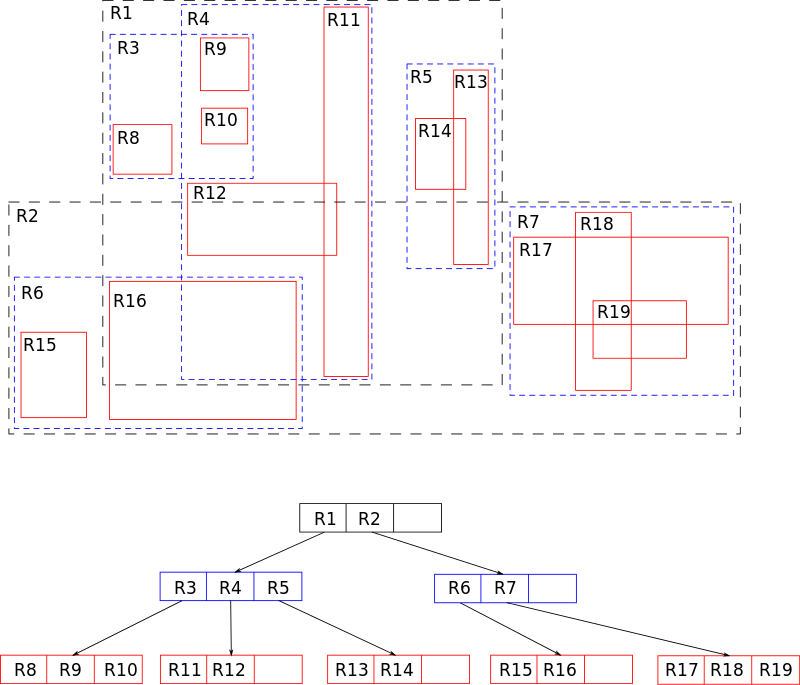
\includegraphics[width=0.8\columnwidth]{./vector_data/img/Rtree}
        \end{center}
    \end{figure}
\end{frame}





    \subsection{Работа с атрибутами}
    
\begin{frame}
    \frametitle{Выбор объектов по атрибутам}
    \begin{figure}[!ht]
        \begin{center}
            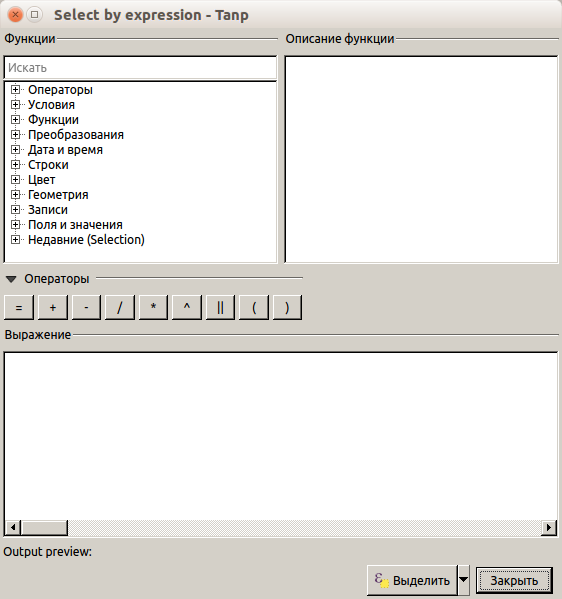
\includegraphics[width=0.6\columnwidth]{./vector_data/img/select_dialog}
        \end{center}
    \end{figure}
\end{frame}

\begin{frame}
    \frametitle{Калькулятор полей}
        \begin{figure}[!ht]
        \begin{center}
            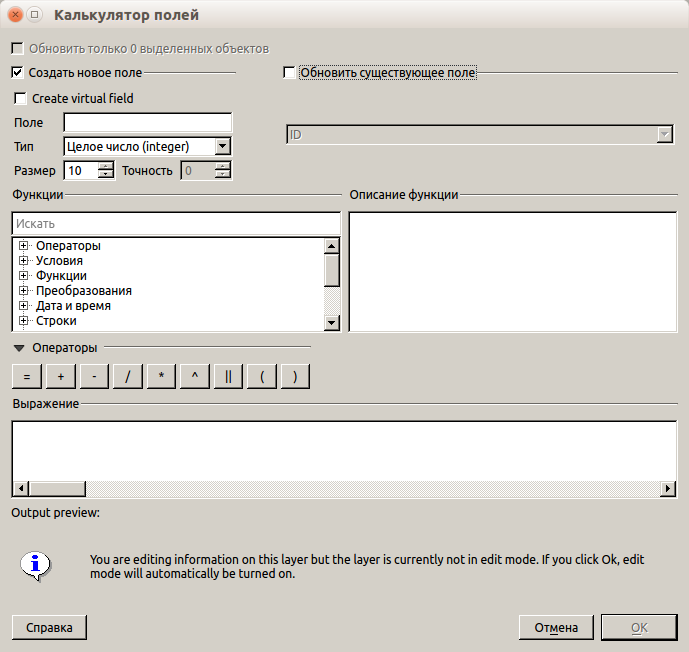
\includegraphics[width=0.6\columnwidth]{./vector_data/img/calculator}
        \end{center}
    \end{figure}
\end{frame}


    \subsection{Инструменты ftools}
    
\begin{frame}[allowframebreaks]
    \frametitle{Анализ}
    \begin{itemize}
        \item Матрица расстояний. Измеряет расстояние между точками двух точечных слоёв и выдает результат в виде (a) квадратной матрицы расстояний, (b) линейной матрицы расстояний, или (c) суммы расстояний. Можно ограничить расчет только для k ближайших точек.
        \item Сумма расстояний в полигонах. Рассчитывает сумму расстояний для линий линейного слоя в пределах каждого полигона другого (векторного полигонального) слоя.
        \item Количество точек в полигонах. Рассчитывает число точек точечного слоя, которые находятся в пределах каждого полигона другого (векторного полигонального) слоя.
        \item Список уникальных значений. Отображает список всех уникальных значений для указанного поля атрибутивной таблицы исходного векторного слоя.
        \item Базовая статистика. Рассчитывает основные статистики (среднее, стандартное отклонение, количество, сумму, коэффициент вариации) для указанного поля.
        \item Анализ близости. Рассчитывает значение близости для оценки степени сгруппированности точек в пределах точечного векторного слоя.

        Наблюдаемое среднее:
        \begin{equation*}
            D_o = \frac{\sum_{i=1}^n d_i}{n},
        \end{equation*}
        где $n$ --- число точек, $d_i$ --- расстояние от точки номер $i$ до ее ближайшего соседа.


        Ожидаемое среднее:
        \begin{equation*}
            D_e = \frac{0.5}{\sqrt{n/A}},
        \end{equation*}
        где $A$ --- площадь изучаемое территории.

        Индекс ближайших соседей:
        \begin{equation*}
            R = \frac{D_o}{D_e}
        \end{equation*}

        Z-показатель:
        \begin{equation*}
            z = \frac{D_o-D_e}{s_e},
        \end{equation*}
        где $S_e = \frac{0.26136}{\sqrt{n^2/A}}$

        \item Средние координаты. Рассчитывает среднеарифметические или средневзвешенные координаты центра для целого векторного слоя или для набора объектов, выбранного на основе уникальные значения из указанного поля.
        \item Пересечение линий. Рассчитывает местонахождения пересечений линий, создавая точечный шейп-файл с точками пересечений.
    \end{itemize}
\end{frame}


\begin{frame}[allowframebreaks]
    \frametitle{Выборка}
    \begin{itemize}
        \item Случайная выборка и Выборка в подмножествах: случайный выбор объектов из таблицы.
        \item Случайные точки. Cоздает псевдо-случайные точки в пределах границ указанного слоя..
        \item Регулярные точки. Создаёт регулярную сетку точек в пределах указаной области и экспортирует их в точечный шейп-файл..
        \item Регулярная сетка. Создаёт линейную или полигональную сетку, основываясь на заданном пользователем интервале..
        \item Пространственная выборка. Выделяет объекты на основе их положения относительно другого слоя, создавая новую выборку или добавляя/отнимая к/от текущей выборки. (Вместо этого инструмента лучше использовать <<Модули/Пространственный запрос>>)
        \item Полигон из границ слоя. Создаёт полигональный слой с единственным прямоугольным полигоном в соответствии с границами исходного растрового или векторного слоя.
    \end{itemize}
\end{frame}


\begin{frame}[allowframebreaks]
    \frametitle{Геообработка}
    \begin{itemize}
        \item Выпуклые оболочки. Создает минимально возможные выпуклые оболочки, или выпуклые оболочки на основе указанного поля.
        \item Буферные зоны. Создает буферные зоны вокруг объектов заданного пользователем размера, или используя размер из значений указанного поля.
        \item Пересечение. Совмещает слои таким образом, что в выходном слое содержатся только участки, в которых оба слоя пересекаются. Аттрибутивная таблица составляется из полей обоих слоев.
        \item Разность. Совмещает слои таким образом, что в выходном слое содержатся только те участки, которые не пересекаются со слоем отсечения.
        \item Cимметрическая разность. Совмещает слои таким образом, что в выходном слое содержатся только те участки, в которых исходные слои не пересекаются. Аттрибутивная таблица составляется из полей обоих слоев.
        \item Отсечение. Совмещает слои таким образом, что в выходном слое содержатся только те участки, которые пересекаются со слоем отсечения.
        \item Объединение. строится слой из пересекающихся объектов указанных слоев, атрибуты объектов объединяются в новой таблице.
        \item Объединение по признаку. Объекты с одинаковыми атрибутами объединяются в один объект.
        \item Удалить осколочные полигоны. Объединяет выделенные объекты с соседним полигоном, площадь или длина общей границы которого наибольшая.
    \end{itemize}
\end{frame}

\begin{frame}[allowframebreaks]
    \frametitle{Обработка геометрии}
    \begin{itemize}
        \item Проверка геометрии. Проверяет полигоны на наличие пересечений, «островов» и неправильного порядка нумерации узлов. (Вместо этого инструмента лучше использовать <<Модули/Проверка топологии>>)
        \item Экспортировать/добавить поле геометрии. Добавляет к слою поле(я) с информацией о геометрии: (XCOORD, YCOORD) для точечного слоя, (LENGTH) для линейного и (AREA, PERIMETER) для полигонального.
        \item Центроиды полигонов. Вычисляет истинные центроиды для каждого полигона исходного полигонального слоя.
        \item Триангуляция Делоне. Рассчитывает и строит (как полигональный шейп-файл) триангуляцию Делоне для исходного точечного слоя.
        \item Полигоны Вороного. Рассчитывает и строит полигоны Вороного для исходного точечного слоя.
        \item Упростить геометрию. Упрощает линии или полигоны при помощи модифицированного алгоритма Дугласа-Пойкера.
        \item Добавить вершины. Добавляет дополнительные вершины к объектам линейного или полиногнального слоя.
        \item Разбить составную геометрию. Преобразует составные объекты (мульти-полигоны или мульти-полилинии) в несколько простых объектов (полигонов или полилиний).
        \item Объединить геометрию в составную. Объединяет несколько простых объектов в один составной на основе значения указанного поля.
        \item Преобразовать полигоны в линии.
        \item Преобразовать линии в полигоны.
        \item Извлечение узлов. Извлекает узлы из линий или полигонов, создавая точечный шейп-файл.
    \end{itemize}

\end{frame}

\begin{frame}
    \frametitle{Управление данными}
    \begin{itemize}
        \item Задать текущую проекцию.
        \item Объединение атрибутов по районам. Присоединяет дополнительные атрибуты к векторному слою на основе пространственного взаимного расположения. Атрибуты из одного векторного слоя присоединяются к атрибутивной таблице другого векторного слоя и экспортируются в шейп-файл.
        \item Разбить векторный слой. Деление слоя на несколько отдельных слоев по указанному атрибуту.
        \item Объединение shape-файлов. Объединяет слои одинакового типа (точки, линии, полигоны) в один слой.
        \item Создать пространственный индекс.
    \end{itemize}
\end{frame}



    \section{Пространственные расширения}
    
\begin{frame}[fragile]
    \frametitle{Базовый запрос на языке SQL}
    \begin{verbatim}
    SELECT поля
    FROM таблицы
    WHERE условие
    \end{verbatim}
\end{frame}

\begin{frame}[allowframebreaks]
    \frametitle{Пространственные расширения языка SQL: базовые операции}
    Базовые операции, применимые ко всем геометрическим типам данных. Например, SpatialReference возвращает базовую систему координат, в которой описана геометрия объекта. К числу распространенных систем координат относятся широко известная система широт и долгот, а также часто используемая система Universal Traversal Mercator (UTM).
    \begin{itemize}
        \item SpatialReference(), ST\_SRID(), SRID(): Возвращает базовую систему координат геометрии
        \item Envelope(), ST\_Envelope(): Возвращает минимальный ортогональный ограничивающий прямоугольник геометрии
        \item Export(), AsText(), ST\_AsText(): Возвращает альтернативное представление геометрии
        \item IsEmpty(), St\_IsEmplty: Возвращает истинное значение, если геометрия является пустым множеством
        \item IsSimple(), ST\_IsSimple(): Возвращает истинное значение, если геометрия является простой (без самопересечений)
        \item Boundary(), ST\_Boundary(): Возвращает границы геометрии (у полигона --- linestring)
        \item Simplyfy(g, tolerance): Возвращает упрощенную геометрию с заданной погрешностью.
    \end{itemize}
\end{frame}


\begin{frame}[allowframebreaks]
    \frametitle{Топологические операции и операции над множествами}
    \begin{itemize}
        \item Equals(g1, g2): Возвращает истинное значение, если внутренние области и
        границы обеих геометрий пространственно равны
        \item Disjoint(g1, g2): Возвращает истинное значение, если границы и внутренняя область g1 и g2 не пересекаются
        \item Intersects(g1, g2): Возвращает истинное значение, если геометрии имеют общие элементы
        \item Touches(g1, g2): Возвращает истинное значение, если границы двух поверхностей пересекаются, а внутренние области --- нет
        \item Crosses: Возвращает истинное значение, если внутренняя область поверхности пересекается кривой
        \item Within(g1, g2): Возвращает истинное значение, если внутренняя область одной геометрии не пересекается с внешней областью другой геометрии g1 в g2
        \item Contains(g1, g2): Проверяет, содержит ли одна геометрия другую g2 в g1.
        \item Overlaps: Возвращает истину, если внутренние области двух геометрий имеют непустое пересечение
    \end{itemize}
\end{frame}

\begin{frame}[allowframebreaks]
    \frametitle{Пространственый анализ}
    \begin{itemize}
        \item Distance: Возвращает кратчайшее расстояние между двумя геометриями
        \item Buffer(geom, R): Возвращает геометрию, содержащую все точки, лежащие на указанном или меньшем расстоянии от данной геометрии
        \item ConvexHull: Возвращает наименьшее выпуклое геометрическое множество, заключающее в себе данную геометрию
        \item Intersection: Возвращает геометрическое пересечение двух геометрий
        \item Difference(g1, g2): Возвращает фрагмент геометрии, который не пересекается с другой геометрией g1 - g2
        \item SymmDiff(g1, g2): Возвращает фрагменты двух геометрий, которые не пересекаются друг с другом
    \end{itemize}
\end{frame}












\section{Основы обработки ДЗЗ}
    \subsection{Излучение и ДЗЗ}
    
\begin{frame}
    \frametitle{Типы ДЗЗ}
    Выделяют следующие типы систем:
    \begin{itemize}
        \item Пассивные: системы регистрируют отраженное от объектов солнычное излучение (оптические сканерные системы). Такие системы собычно содержат несколько каналов, каждый из которых регистрирует излучение в определенной зоне спектра.
        \item Активные: сами излучают сигнал (в области микроволнового излучения) и регистрируют вернувшийся назад отклик (радарные системы). Основное преимущество таких систем перед пассивными --- они не звисят от погоды и облачности.
    \end{itemize}
\end{frame}

\begin{frame}
    \frametitle{Излучение и атмосферные эффекты}
    \begin{figure}[!ht]
        \begin{center}
            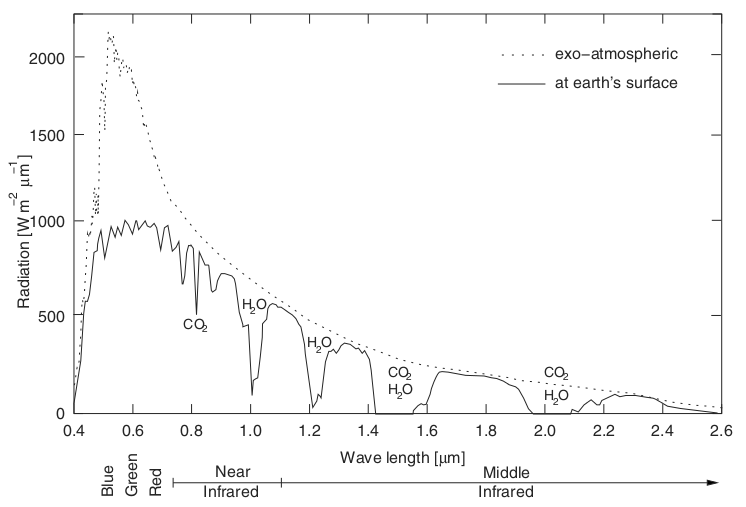
\includegraphics[width=1.0\columnwidth]{./remote_sensing/img/solar_radiation}
        \end{center}
        \caption{\tiny Neteler, Markus. Open source GIS. No. 6. SAGE Publications, 2010.}
    \end{figure}
\end{frame}
\note{
рассказать о том, как изменяется уровень излучения проходя через атмосферу. О необходимости коррекции атмосферных эффектов
}

\begin{frame}
    \frametitle{Отраженное излучение различных классов объектов}
        \begin{figure}[!ht]
        \begin{center}
            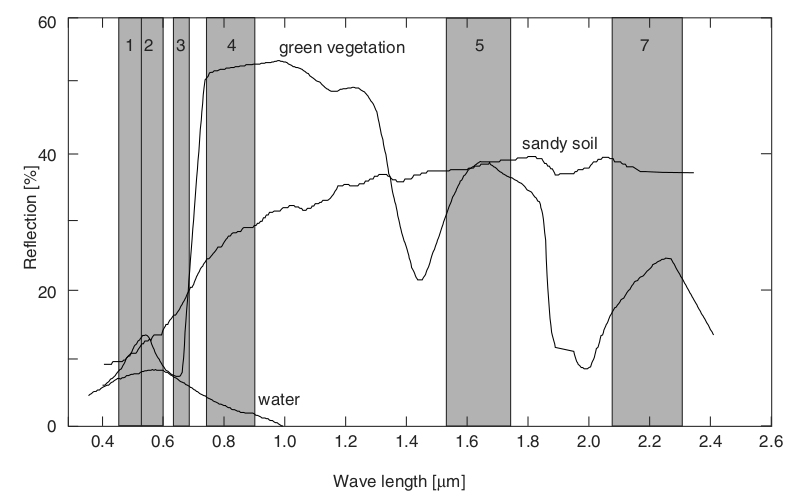
\includegraphics[width=1.0\columnwidth]{./remote_sensing/img/reflectance}
        \end{center}
        \caption{\tiny Neteler, Markus. Open source GIS. No. 6. SAGE Publications, 2010.}
    \end{figure}
\end{frame}
\note{
О том, что разные объекты отражают по разному. Что поведение линий (см. рис.) очень специфично для объектов. Что существуют специальные спектральные библиотеки.
}

\begin{frame}
    \frametitle{Данные, получаемые от оптических систем}
    Растровые изображения, характеризуются разрешением:
    \begin{itemize}
        \item пространственным;
        \item спектральным;
        \item радиометрическим.
    \end{itemize}
\end{frame}

\begin{frame}
    \frametitle{Примеры}
    \begin{figure}[!ht]
        \begin{center}
            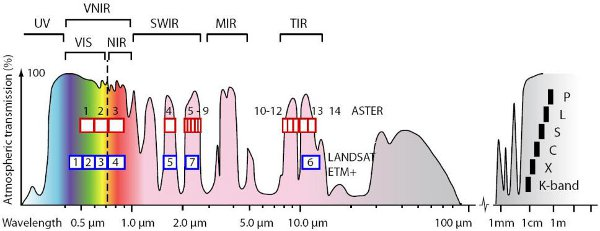
\includegraphics[width=1.0\columnwidth]{./remote_sensing/img/bands}
        \end{center}
        \caption{\tiny Kenneth A. Duda, Michael Ramsey, Rick Wessels and Jonathan Dehn (2009). Optical Satellite Volcanеo Monitoring: A Multi-Sensor Rapid Response System, Geoscience and Remote Sensing, Pei-Gee Peter Ho (Ed.)}
    \end{figure}
    Ландсат-5 : 30-метровое разрешение, однобайтовое радиометрическое разрешение.
\end{frame}

\begin{frame}
    \frametitle{Пространство признаков}
    \begin{figure}[!ht]
        \begin{center}
            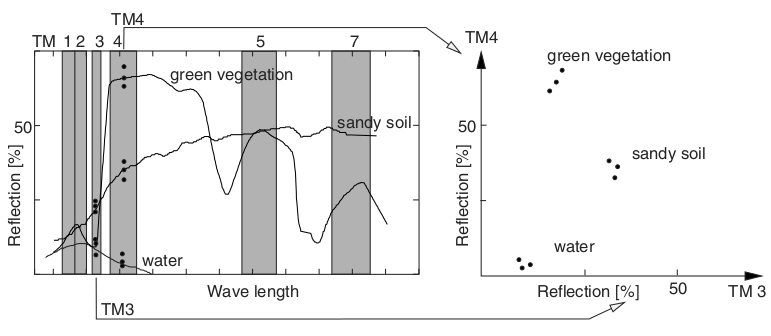
\includegraphics[width=1.0\columnwidth]{./remote_sensing/img/feature_space}
        \end{center}
        \caption{\tiny Neteler, Markus. Open source GIS. No. 6. SAGE Publications, 2010.}
    \end{figure}

\end{frame}


    \subsection{Предобработка данных}
    
\begin{frame}
    \frametitle{Радиометрическая коррекция}
    Данные, которые приходят со спутника измеряются <<в попугаях>> ($DN$), поскольку они сжаты в определенный диапазон значений.

    Для того, чтобы получить реальное зарегистрирванное сенсором излучение ($L_j$), нужно рассчитать его по формуле:

    \begin{equation*}
        L_j = gain_j DN_j + bias_j
    \end{equation*}
    где параметры $gain_j$ и $bias_j$ указываются в метаданных.

    На этом часто останавливаются (особенно, если анализируется один снимок). Если нужно учесть атмосферные эффекты (анализ разновременных снимков), выполняют атмосферную коррекцию.
\end{frame}

\begin{frame}[allowframebreaks]
    \frametitle{Атмосферная коррекция}
    Технологию можно прочитать подробнее в Шовенгердт Р.А. Дистанционное зондирование. Модели и методы обработки изображений. М.: Техносфера, 2010. - 560 с. - ISBN: 978-5-94836-244-1; (перевод книги Robert A. Schowengerdt Models and Methods for Image Processing ISBN: 978-0-12-369407-2)

    Полная атмосферная коррекция выполняется редко, поскольку для этой процедуры требуется знать состояние атмосферы на всей площади снимка, а это сложно. Поэтому состояние атмосферы оценивают по самим снимкам и полученные оценки используют для коррекции. Более-менее стандартная схема работы такова:

Обозначения: $b$ --- номер канала; $DN_b$ --- значения пикселей снимков в попугаях; зарегистрированное датчиком излучение для канала $b$ обозначим $L^s_b$.
\begin{enumerate}
    \item Преобразование из попугаев в излучение производится линейно:
    $$L^s_b = gain_bDN_b +bias_b$$
    параметры преобразования берутся из метаданных снимка.
    \item Собственно атмосферная коррекция. Излучение у поверхности Земли ($L_b$) в точке $(x,y)$ при предположении, что отраженным от Земли рассеяным излучением можно пренебречь, рассчитывается:
    $$L_b(x,y) = \frac{L^s_b(x,y) - L_b^{sp}}{t_{vb}},$$
    где $t_{vb}$ --- спектральный коэффициент пропускания атмосферы (табличное значение, зависит от длины волны), а $L^{sp}_b$ --- плотность потока рассеянного излучения (не дошедшего до Земли и вернувшегося на датчик). Для сцен с однородным рельефом и датчиков, снимающих в надире обычно считается постоянной на всей площади снимка (но зависит от длины волны).
    \item Оценка плотности потока рассеянного излучения $L^{sp}_b$. Способов много разной степени сложности. Простой но действенный --- найти черный объект(ы) и вычесть из всех пикселей значения яркости пикселей, соответствующих черному объекту(ам)
    \item Поправка на угол восхождения Солнца и расчет отражательной способности:
    $$\rho_b(x,y) = \frac{\pi L_b(x,y)} {t_{sb}E^0_b\cos(\Theta(x,y))},$$
    где $E^0_b$ --- спектральная плотность энергетической освещенности на верней границе атмосферы (хорошо известная величина), $\Theta$ --- угол направления на Солнце.

    Как считать излучение у поверхности Земли показано на шаге 2, спектральная плотность потока на верхней границы атмосферы --- табличная величина, угол падения излучения (зависит от угла восхождения Солнца и рельефа). Остается коэффициент пропускания атмосферы $t_{sb}$, который как-то нужно оценить (в идеале должен измеряться в момент съемки).
\end{enumerate}

\end{frame}


    \subsection{Классификация}
    
\begin{frame}
    \frametitle{Задача классификации}
    Есть входные данные --- излучение зарегистрированное в разных каналах: $(x_1, x_2, \dots, x_n)$ нужно отнести данную
    точку к тому или иному классу объектов.

    Хорошо изученная задача. Множество методов решения. Два основных подхода к решению:
    \begin{itemize}
        \item Контролируемая классификация (обучение с учителем).
        \item Неконтролируемая классификация (обучение без учителя).
    \end{itemize}
\end{frame}


\section{Взаимодейсвие с GRASS}
    \subsection{Обзор GRASS GIS}
    
\begin{frame}
\frametitle{GRASS: Geographic Resources Analysis Support System}
\begin{itemize}
\item Разрабатывается с 1984 года (USA-CERL). Все это время была открытой ГИС.
\item Кроссплатформенная: доступны версии для GNU/Linux, MS-Windows, Mac OSX, SUN, \dots; 32/64 битные системы.
\item Хорошо документирована, большие коллекции данных. Коммерческая поддержка.
\item Русское зеркало: \href{http://grass.gis-lab.info/index.php}{http://grass.gis-lab.info/index.php}
\end{itemize}
\begin{figure}[!ht]
          \begin{center}
            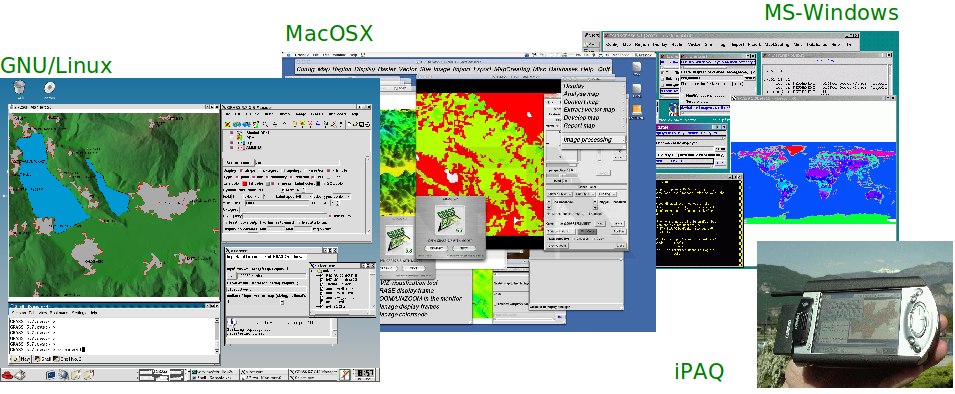
\includegraphics[width=0.8\columnwidth]{./grass/img/platforms.png}
        \end{center}
\end{figure}
\end{frame}

\begin{frame}
\frametitle{GRASS GIS это:}
\begin{multicols}{2}
\begin{itemize}
\item Растровая 2.5D/3D ГИС
\item  Вектроная 2D/3D топологическая ГИС
\item Анализ и обработка графов
\item Система обработки изображений
\item Система 2D и 3D визуализации
\item Поддержка баз данных:dbf, PostgreSQL, MySQL и sqlite. MS SQL, Oracle (ODBC)
\item Поддерживает все распространенные растровые и векторные форматы
\end{itemize}
\begin{figure}[!ht]
          \begin{center}
            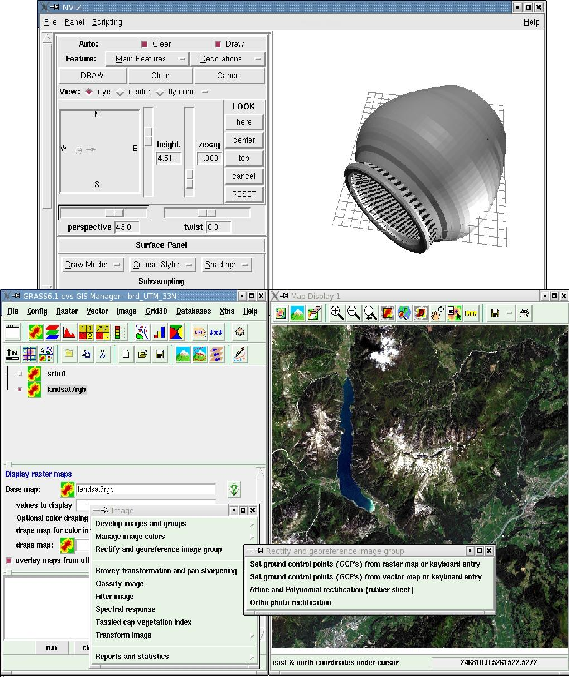
\includegraphics[width=\columnwidth]{./grass/img/views.png}
        \end{center}
\end{figure}
\end{multicols}
\end{frame}


\begin{frame}
\frametitle{Типы пространственных данных}
\begin{itemize}
\item 2D Растровые данные, включая спутниковые снимки и аэрофотосъемку
\item 3D (Voxel) данные
\item  2D/3D векторные данные с поддержкой топологии
\end{itemize}
\begin{figure}[!ht]
          \begin{center}
            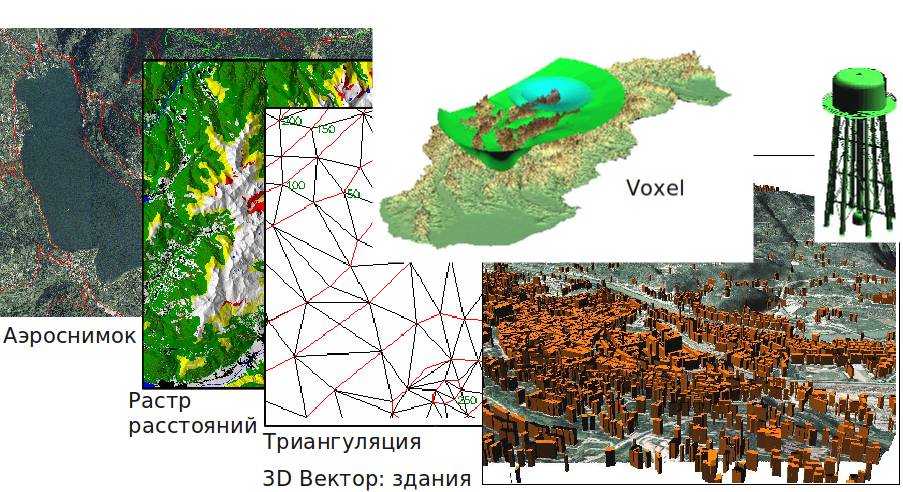
\includegraphics[width=0.8\columnwidth]{./grass/img/datatypes.png}
        \end{center}
\end{figure}
\end{frame}

\begin{frame}
\frametitle{Растровые данные}
\begin{itemize}
\item Растровые данные: представляют собой сетку пикселей, содержащих некоторые значения какого-либо параметра (высота, концентрация и т.п.).
\item Воксельные данные: обобщение растра, переход к трем измерениям.
\end{itemize}
\begin{multicols}{2}
\begin{figure}[!ht]
          \begin{center}
            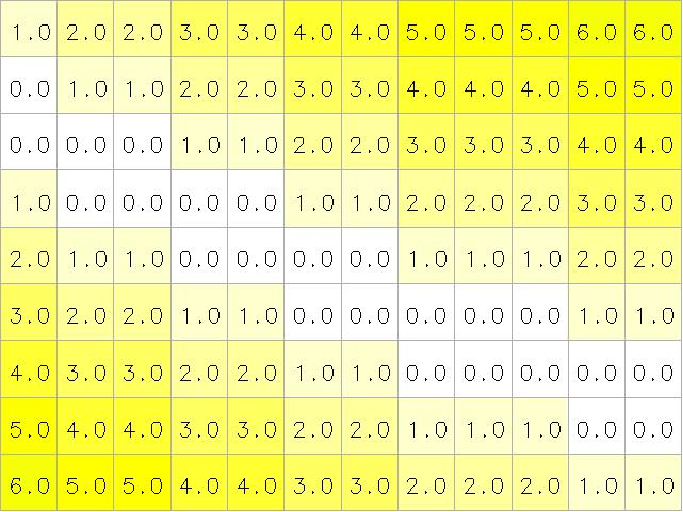
\includegraphics[width=\columnwidth]{./grass/img/raster_model.png}
        \end{center}
\end{figure}
\begin{figure}[!ht]
          \begin{center}
            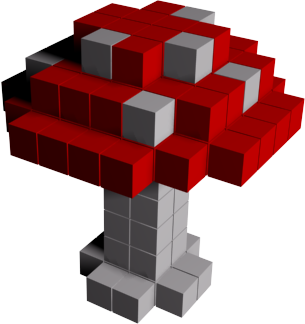
\includegraphics[width=0.7\columnwidth]{./grass/img/voxel_model.png}
        \end{center}
\end{figure}
\end{multicols}
\end{frame}

\begin{frame}
\frametitle{Векторные данные}
\begin{figure}[!ht]
          \begin{center}
            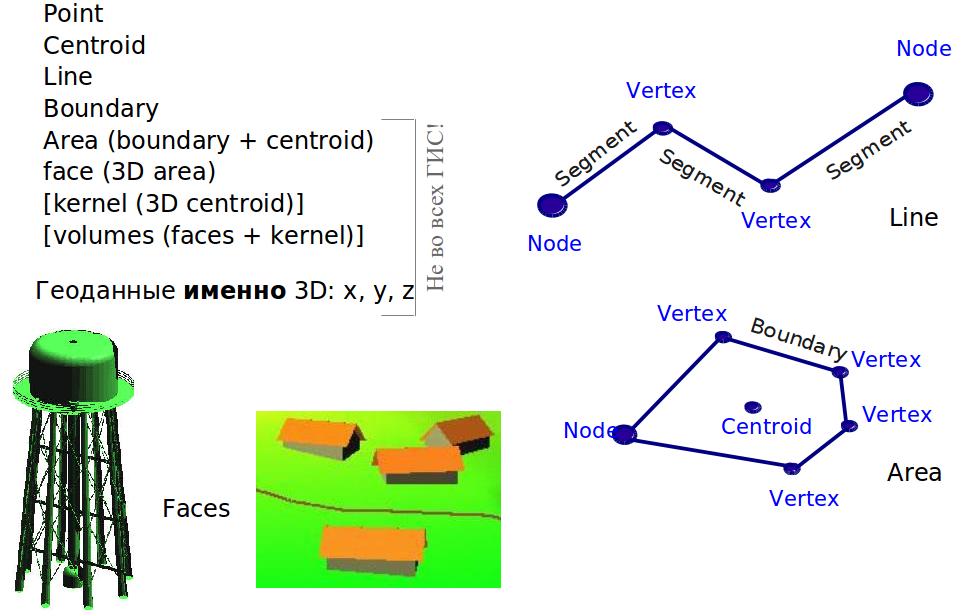
\includegraphics[width=\columnwidth]{./grass/img/vector_data.png}
        \end{center}
\end{figure}
\end{frame}


\begin{frame}
\frametitle{Взаимодействие с другими программами/системами}
\begin{figure}[!ht]
          \begin{center}
            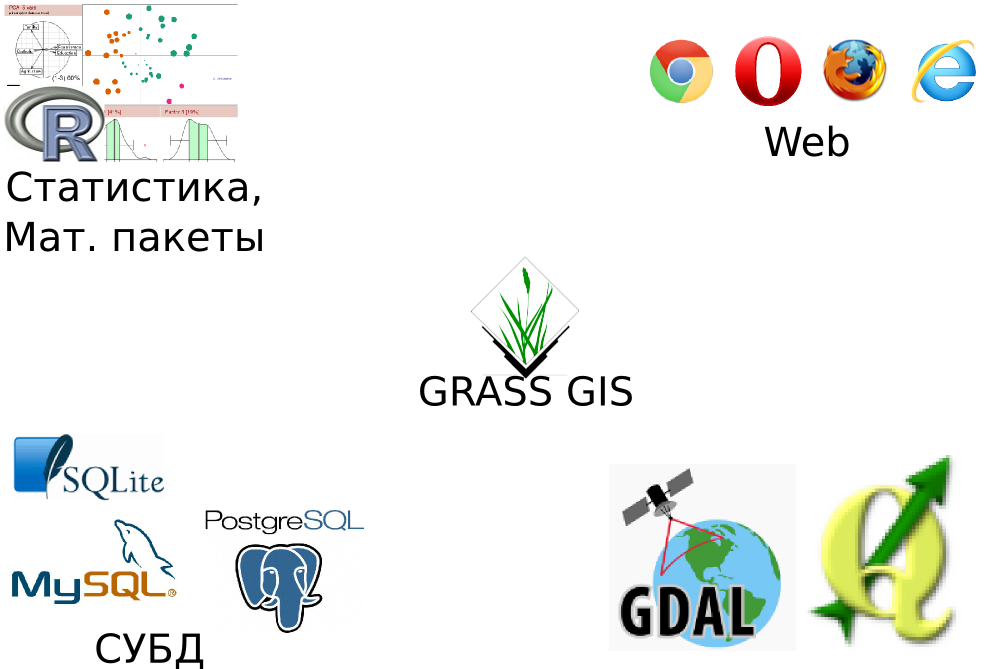
\includegraphics[width=0.9\columnwidth]{./grass/img/grass_prog.png}
        \end{center}
\end{figure}
\end{frame}



    \subsection{Правка топологии на базе инструментов GRASS}
    
\begin{frame}[fragile]
    \frametitle{Инструменты правки топологии в GRASS}
    Основные инструменты:
    \begin{itemize}
        \item v.build --- построение топлогии (вызывается автоматически при импорте объектов);
        \item v.clean --- основной инструмент обработки топологии:
        \begin{verbatim}
        v.clean input=name output=name
        [type=string[,string,...]]
        [error=name]
        tool=string[,string,...]
        [thresh=float[,float,...]]
        \end{verbatim}
    \end{itemize}
\end{frame}

\begin{frame}[fragile]
    \frametitle{Основные параметры v.clean}
    \begin{verbatim}
    v.clean input=name output=name
    [type=string[,string,...]] [error=name]
    tool=string[,string,...] [thresh=float[,float,...]]
    \end{verbatim}
    \begin{itemize}
        \item input: название входной векторной карты, для которой проверяется/чистится топология
        \item output: название выходной векторной карты, в которой сохраняется результат
        \item type: тип объектов, которы обрабатываются (point, line, boundary, centroid, area, face, kernel). По умолчанию: point, line, boundary, centroid, area
        \item error: название выходной карты, в которую записываются ошибки
        \item tool: инструменты обработки
        \item thresh: пороговые значения для инструментов обработки топологии
    \end{itemize}
\end{frame}

\begin{frame}[allowframebreaks]
    \frametitle{Tool}
    \begin{itemize}
        \item break: Разбивать линии на пересечениях. Также разбивает линнии, если они образуют <<сплющеные>> петли. Например, линия (0 0, 1 0, 0 0) будет разбита на две: (0 0, 1 0) и (1 0, 0 0).
        \item snap: Притягивание вершин друг к другу в пределах заданного порога. При большом пороге может повреждать топологии при type=boundary. (Такие <<притянутые>> границы могут быть обработаны последовательностью break,rmdupl,rmsa).
        \item rmdangle: Удаление <<висящих>> узлов.
        \item chdangle: Изменение типа <<висящего>> узла с границы на линию.
        \item rmbridge: Удаление <<мостов>> между островами.
        \item chbridge: Изменение типа <<моста>> между островами с границы на линию.
        \item rmdupl: Удаляет дубликаты геометрий. (Категории!!!) Удобно использовать после инструмента break.
        \item rmdac: Удаляет дубликаты центроидов (они могут появляться после удаления границ).
        \item bpol: Чистит топологию при импорте из нетопологического формата. Границы разбиваются в каждой точке, общей для двух геометрий. (Похоже на break, но работает быстрее, зато требует больше памяти). После применения стоит прогнать rmdupl.
        \item prune: Прореживает узлы, которые лежат ближе указанного порога. Если чистятся границы, то топология сохраняется (отличие от snap).
        \item rmarea: Удаляет площади, которые меньше заданного порога. Удаление площади происходит за счет удаление наиболее протяженной общей границы и удаления всех неразделяемых границ.
        \item rmline: Удаление всех линий нулевой длины.
        \item rmsa: Удаление <<щелей>>:
        \begin{figure}[!ht]
            \begin{center}
                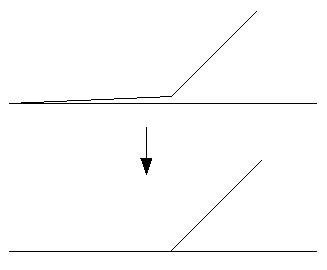
\includegraphics[width=0.4\columnwidth]{./grass/img/v_clean_rmsa}
            \end{center}
        \end{figure}
    \end{itemize}
\end{frame}

\begin{frame}[fragile]
    \frametitle{Генерализация инструментами GRASS GIS}
    \begin{itemize}
        \item Генерализация в момент импорта данных (уделение полигонов меньших заданого порога, <<прищелкивание>> узлов):
\begin{verbatim}
v.in.ogr -e dsn=regions2010.shp out=regions
    min_area=1 snap=100
\end{verbatim}


        \item v.clean:
\begin{verbatim}
v.clean in=regions out=sipmle type=boundary
    tool=prune,rmarea thresh=2000,4000000
\end{verbatim}
        \item v.generalize: специальный инструмент генерализации:
\begin{verbatim}
v.generalize input=name output=name
[type=string[,string,...]]
method=string threshold=float
...
[where=sql_query]
\end{verbatim}
    \end{itemize}
\end{frame}

\begin{frame}[allowframebreaks]
    \frametitle{Обзор методов упрощения геометрий v.generalize}
    \begin{itemize}
        \item Инструмент reduction -- самый простой алгоритм из представленных, удаляет точки линии, которые лежат около друг-друга ближе, чем на заданное пороговое расстояние. Таким образом, алгоритм использует один задаваемый пользователем параметр -- максимально допустимое расстояние, при котором точки считаются идентичными.
        \item Инструмент douglas реализует классический алгоритм Дугласа-Пекера. Инструмент принимает один параметр -- максимальное допустимое отклонение генерализованной линии от изначальной.
        \item Инструмент douglas\_reduction представляет собой модификацию алгоритма Дугласа-Пекера, в которой задается дополнительный параметр -- желаемое количество точек генерализованной линии, которое требуется достичь (измеряется в процентах по сравнению с количеством точек исходной линии).
        \item Инструмент lang также похож на алгоритм Дугласа-Пекера. Основное отличие состоит в том, что lang представляет собой не рекурсивный алгоритм. Поэтому, во избежание рекурсии алгоритм использует дополнительный параметр (look\_ahead), задающий число точек, которые требуется просмотреть
        \item Инструмент reumann использует коридор из двух параллельных линий заданной ширины. Для построения коридора берутся две последовательные точки линии и в направлении, заданном отрезком между точками строится коридор. Далее определяется место выхода линии за границы коридора, в результате точки и сегменты исходной линии, которые попали внутрь коридора, замещаются одним сегментом и процесс повторяется со следующей парой непросмотренных точек. Параметр алгоритма -- ширина коридора.
    \end{itemize}
\end{frame}

\begin{frame}[allowframebreaks]
    \frametitle{Обзор методов упрощения геометрий v.generalize}
    \begin{itemize}
        \item Инструмент boyle сглаживает методом скользящего среднего: алгоритм расчитывает среднее между look\_ahead последовательных точек линии, начиная с текущей. Таким образом алгоритм использует единственный параметры -- ширину окна look\_ahead.
        \item Инструмент sliding\_averaging сначала расчитывает средние кординаты для look\_ahead точек до и look\_ahead после текущей точки (т.е. усредняется 2*look\_ahead+1 точка), полученные координаты запоминаются. Целевая (сглаженная) точка помещается на отрезке, проведенном между исходной и усредненной точкой, местоположение на котором задается параметром slide (0 -- исходная точка, 1 -- усредненная точка). Соответственно, алгоритм использует два параметра: ширину окна look\_ahead и степень сдвига slide.
        \item Инструмент distance\_weighting аналогичен предыдущему, за исключением того, что усредненная точка расчитывается методом взвешенного среднего. Как и sliding\_averaging, алгоритм использует два параметра: ширину окна look\_ahead и степень сдвига slide.
        \item Эрмитова интерполяция --- алгоритм на базе кубический сплайнов.
        \item \dots
    \end{itemize}
\end{frame}






    \subsection{Сетевой анализ в GRASS GIS}
    
%~ \begin{frame}[fragile]
    %~ \frametitle{Инструменты GRASS для работы с сетями}
    %~ \begin{itemize}
        %~ \item v.net: создание сети.
        %~ \item v.net.iso: изодистанции
        %~ \item v.net.path кратчайший путь
    %~ \end{itemize}
%~ \end{frame}

% Конвертируем полигоны в линии
% v.type roads out=roads1 type=boundary,line,centroid,point
% v.clean input=roads1@PERMANENT type=line tool=snap,break,rmdupl,rmsa thresh=20,0,0,0 output=test --o
%  v.category test opt=report
%  v.edit test type=point tool=delete cat=1-400

% Считаем изолинии:
% v.net streets points=schools out=streets_net op=connect thresh=200
% v.net.iso in=streets_net out=streets_net_iso ccats=1-1000000 nlayer=2 costs=200,400,600,800
% v.category streets_net_iso opt=report # 5 cats

% Считаем кратчайший путь между двумя узлами:
% 1 - ID, растояние считается от узла категории 15 до узла категории 21
% номер категории можно узнать, если включить отображение "Display category numbers" в менеджере слоев и показать категории со слоя 2 (v.net op=connect складывает присоединенные узлы во второй слой)
% echo "1 15 21" | v.net.path streets_net out=spath


% Linear reference system (LRS)
% v.lrs.create создание системы
% v.lrs.label to create stationing on LRS
% v.lrs.segment to create points/segments from LRS
% v.lrs.where to find the line ID





    \subsection{Солнечная освещенность}
    
\begin{frame}[fragile,allowfrimebreaks]
    \frametitle{Солнечная освещенность}
    r.sunmask служит для расчета положения солнца и прогноза карты теней (алгоритм SOLPOS2, учитывает рефракцию атмосферы):
    \begin{verbatim}
r.sunmask -s --v aster_gdem out=dummy
    year=2014 month=11 day=13 hour=14 minute=25
    sec=0 timezone=+3
    \end{verbatim}

    \begin{verbatim}
r.sunmask --v aster_gdem out=shadows
    year=2014 month=11 day=13 hour=14 minute=25
    sec=0 timezone=+3
    \end{verbatim}
\end{frame}



    \subsection{Обработка данных ДЗЗ инструментами GRASS}
    
\begin{frame}
    \frametitle{Обработка данных ДЗЗ инструментами GRASS}
    \begin{itemize}
        \item Здесь речь пойдет в первую очередь о данных, полученных в
        результате аэро- и космосъемки оптических систем (фото- и сканерная съемка).
        \item С точки зрения GRASS, согласно ее внутреннему представлению данные (аэро)космосъемки являются обычными растрами, как следствие команды обработки растровых данных широко используются для работы с данными ДЗЗ.
        \item Существуют специальные команды (модули), разработанные именно для обработки данных ДЗЗ.
    \end{itemize}
\end{frame}

\subsection{Импорт данных}
\begin{frame}
    \frametitle{Импорт данных}
    \begin{enumerate}
        \item Импорт снимков производится точно также, как и импорт других растровых материалов.
        \item Основная особенность импорта данных относится к многоканальным снимкам: для некоторых модулей обработки изображений необходимо предварительно собрать изображения анализируемой сцены в группу. Это можно сделать при помощи модуля \lstinline!i.group!. К группе можно присоеденить и другие растры, не обязательно полученные в результате космо/аэросъемки.
    \end{enumerate}
\end{frame}

\begin{frame}
    \frametitle{Особенности ортокоррекции в GRASS}
    Для выполнения ортокоррекции GRASS предоставляет следующие модули:
    \begin{enumerate}
        \item \lstinline!i.group!, \lstinline!i.target!: создают группу изображений, задают целевой проект/набор.
        \item \lstinline!i.points!: позволяет указать точки для привязки изображений.
        \item \lstinline!i.rectify!: производит трансформацию изображений.
    \end{enumerate}

    По своей сути данный инструмент --- инструмент привязки растров. Он часто используется для обработки данных аэросъемки, но плохо приспособлен для сканерных систем.
\end{frame}


\begin{frame}[fragile,shrink]
    \frametitle{Радиометрическая коррекция}
    \begin{block}{Радиометрическая коррекция}
    При регистрации данных физические величины яркости каналов приводятся к диапазону [Q\_MIN,Q\_MAX] (преобразование L -> DN). Исходные максимальные и минимальные значения яркостей обычно приводятся в метаданных к снимку.

    Обратное преобразование (DN->L) производится по формуле:
    \begin{equation*}
        L = \frac{LMAX - LMIN}{Q\_MAX-Q\_MIN} (DN-Q\_MIN) + LMIN
    \end{equation*}
    \end{block}
    Например, для Landsat5 по третьему каналу:
    \begin{lstlisting}
        LMAX_BAND3 = 264.000        LMIN_BAND3 = -1.170
    \end{lstlisting}
    Соответственно, калибровка производится на основе калькулятора растров:
    \begin{lstlisting}
r.mapcalc "b3 = (264.0+1.17)*(L5_B30-1)/254 + 1.17"
    \end{lstlisting}
\end{frame}

\begin{frame}[fragile]
    \frametitle{Атмосферная коррекция}
    В GRASS есть модуль атмосферной коррекции \lstinline!i.attcor!, в котором реализован алгоритм 6S --- Second Simulation of Satellite Signal in the Solar Spectrum.

    Существуют специальные модули для работы с данными Landsat:
    \begin{itemize}
        \item \lstinline!i.landsat.toar!: расчет отражательной способности (на верхней границы атмосферы).
        \item \lstinline!i.landsat.dehaze!: удаление дымки (AddOns).
    \end{itemize}
\end{frame}

\begin{frame}
    \frametitle{Отображение композитных снимков}
    В ГИС-менеджер встоен инструмент построения RGB- и HIS-изображений на основе трех компонент цвета. Кроме того существуют специальные модули преобразования одного представления цвета в другое и повышения разрешения снимков:
    \begin{itemize}
        \item \lstinline!i.rgb.his!: преобразование rgb -> his.
        \item \lstinline!i.his.rg!: преобразование his -> rgb.
        \item \lstinline!i.fusion.brovey!: улучшение пространственного разрешения.
    \end{itemize}

    Для создания мозаик из снимков разработан специальный модуль: \lstinline!i.image.mosaic!. Ограничение модуля --- используются до 4-х снимков.
\end{frame}


\begin{frame}
    \frametitle{Особенности использования методов классификации в GRASS}
    Классификация в GRASS происходит в два этапа:
    \begin{enumerate}
        \item Расчет сигнатур --- характеристик классов. Классы могут быть как заданными пользователем, так и выделяться автоматически (контролируемая и неконтролируемая классификации).
        \item Классификация неклассифицированных пикселей по сигнатурам, определенным на первом этапе.
    \end{enumerate}

    Это позволяет комбинировать различные алгоритмы построения сигнатур и различные алгоритмы классификации.
\end{frame}

\begin{frame}
    \frametitle{Основные методы классификации в GRASS}
    GRASS поддерживает следующие методы классификации:
    \begin{itemize}
        \item Классификация на основе попиксельного радиометрического анализа:
            \begin{itemize}
                \item Контролируемая классификация:  \lstinline!i.cluster! (кластеризация), затем \lstinline!i.maxlik! (классификация методом максимального правдоподобия).
                \item Неконтролируемая классификация: \lstinline!i.gensig! (неинтерактивный расчет сигнатур по заданным пользователем образцам)/\lstinline!i.class!(интерактивный расчет сигнатур и определение образцов), затем \lstinline!i.maxlik! (метод максимального правдоподобия).
            \end{itemize}
        \item Классификация на основе анализа геометрических и радиометрических характеристик:
            \begin{itemize}
                \item Контролируемая классификация:  \lstinline!i.gensigset!(неинтерактивный расчет сигнатур по заданным пользователем образцам), затем \lstinline!i.smap!(последовательная оценка апостериорного максимума).
            \end{itemize}
    \end{itemize}
\end{frame}

\begin{frame}[fragile]
    \frametitle{Пример: i.smap}
    Рассмотрим процедуру контролируемой классификации. Для примера выберем классификацию на основе \lstinline!i.smap! данных Landsat~5. Для определенности пусть каналы снимка с 1-го по 7-й представлены растрами с названиями L1, L2,\dots, L7, а отклассифицированные образцы находятся в растре train. Тогда:
    \begin{enumerate}
        \item Создадим группу изображений \lstinline!landsat!:
        \begin{lstlisting}
i.group group=landsat subgroup=all \
    input=L1,L2,L3,L4,L5,L6,L7
        \end{lstlisting}
        \item Рассчитаем сигнатуры по образцам:
        \begin{lstlisting}
i.gensigset trainingmap= group=landsat \
    subgroup=all signaturefile=allsig
        \end{lstlisting}
        \item Произведем классификацию:
        \begin{lstlisting}
i.smap group=landsat subgroup=all \
    signaturefile=allsig output=result
        \end{lstlisting}
    \end{enumerate}
\end{frame}

\begin{frame}
    \frametitle{Обра\-бот\-ка раз\-новре\-мен\-ных данных: r.series}
    Для агрегации информации по временной серии растров/изображений используется команда \lstinline!r.series!. Она позволяет расчитать следующие параметры:
    \begin{itemize}
        \item среднее значение,
        \item медиану
        \item моду,
        \item минимум и максимум,
        \item ранг (max - min),
        \item дисперсию,
        \item стандартное отклонение,
        \item параметры линейной регрессии зависимости растров от времени,
        \item \dots
    \end{itemize}
\end{frame}

\begin{frame}
    \frametitle{Метод главных компонент}
    При помощи модуля \lstinline!i.pca! можно произвести трансформацию нескольких снимков по методу главных компонент. Данный метод может быть использован для:
    \begin{itemize}
        \item Выделения наиболее важной информации в серии снимков.
        \item Поиска изменений на разновременных снимках.
    \end{itemize}
\end{frame}

\begin{frame}
    \frametitle{Текстурные признаки}
    \begin{itemize}
        \item r.neighbours
        \item r.texture
    \end{itemize}

\end{frame}


% На примере данных gisconf

% Контролируемая:
% Создать вектор train
% v.to.rast train out=train use=attr col=id
% i.group group=landsat subgroup=all input=B10,B20,B30,B40,B50,B60,B70
% i.gensigset trainingmap=train group=landsat subgroup=all signaturefile=allsig
% i.smap group=landsat subgroup=all signaturefile=allsig output=result

% неконтролируемая:
% i.cluster group=landsat subgroup=all sigfile=sig_clust classes=10
% i.maxlik group=landsat subgroup=all sigfile=sig_clust class=result_clust

% Работа по текстурам
% r.mapcalc "ph = if(photo>255, 255, photo)" # текстуры не работают с > 255 значений

%~ r.texture -d inp=ph prefix=d  --o
%~ r.texture -k inp=ph prefix=k  --o
%~ r.texture -c inp=ph prefix=c  --o
%~ r.texture -d inp=ph prefix=d  --o
%~ r.texture -v inp=ph prefix=v  --o
%~ r.texture -e inp=ph prefix=e  --o
%~ r.texture -a inp=ph prefix=a  --o
%~ r.neighbors --help
%~ r.neighbors in=ph out=avg met=average
%~ r.neighbors in=ph out=variance met=var
%~ r.neighbors in=ph out=var met=variance
%~ r.neighbors in=ph out=div met=diversity
%~ r.neighbors in=ph out=range met=range
%~ i.group textures sub=all inp=a_ASM_0,a_ASM_135,a_ASM_45,a_ASM_90,avg,c_Contr_0,c_Contr_135,c_Contr_45,c_Contr_90,d_DV_0,d_DV_135,d_DV_45,d_DV_90,div,e_Entr_0,e_Entr_135,e_Entr_45,e_Entr_90,k_Corr_0,k_Corr_135,k_Corr_45,k_Corr_90,range,v_Var_0,v_Var_135,v_Var_45,v_Var_90,var
%~
%~ v.to.rast in=train out=train use=attr col=id
%~ i.gensigset trainingmap=train group=textures subgroup=all signaturefile=allsig
%~ i.pca inp=a_ASM_0,a_ASM_135,a_ASM_45,a_ASM_90,avg,c_Contr_0,c_Contr_135,c_Contr_45,c_Contr_90,d_DV_0,d_DV_135,d_DV_45,d_DV_90,div,e_Entr_0,e_Entr_135,e_Entr_45,e_Entr_90,k_Corr_0,k_Corr_135,k_Corr_45,k_Corr_90,range,v_Var_0,v_Var_135,v_Var_45,v_Var_90,var  out=pca
%~ i.group pca sub=tree inp=pca.1,pca.2,pca.3
%~ i.gensigset trainingmap=train group=pca subgroup=tree signaturefile=allsig
%~ i.smap group=pca subgroup=tree signaturefile=allsig output=result







%~
%~ \section{QGIS Browser.}
%~ 
\begin{frame}
    \frametitle{QGIS Browser}
    \begin{figure}[!ht]
        \begin{center}
            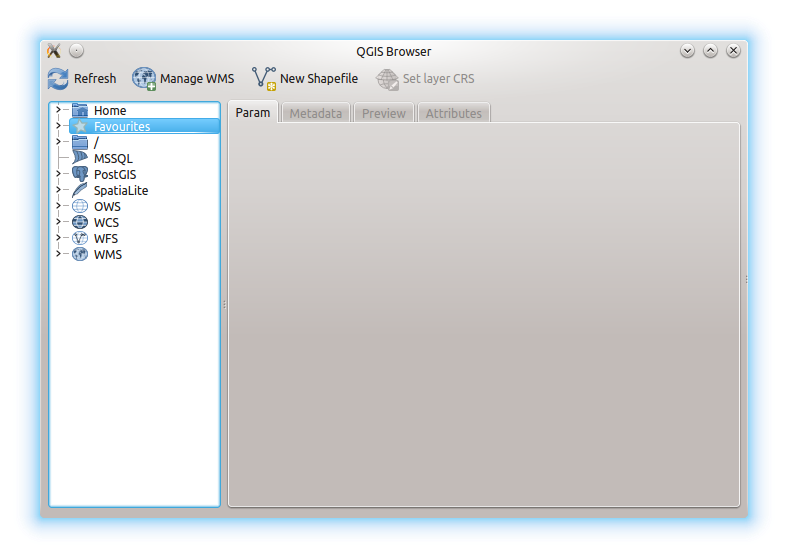
\includegraphics[width=0.75\columnwidth]{./qgis_browser/img/qgis_browser_interface.png}
        \end{center}
        \caption{Окно QGIS Browser.}
    \end{figure}


\end{frame}
\note{
Рассказать, для чего используется QGIS Browser.

Например, форматы данных часто содержат
несколько файлов слайды \ref{MapInfoVectorFormat}, \ref{ShpVectorFormat}, работать с ними нужно умеючи.
Сложность прячет
}



\section{Практика}
    %~ \subsection{Интерфейс QGIS}
    %~ \input{practic/interface.tex}
%~
    %~ \subsection{Системы координат}
    %~ 
\begin{frame}
    \frametitle{Преобразование координат}
    \begin{itemize}
        \item Отрыть слой административного деления AdminWGS84.
        \item Определить зону Гаусса-Крюгера, в которой лежит основная часть территории.
        \item Произвести перепроецирование карты в соответствующую зону Г-К на эллипсоиде Крассовского.
        \item Определить зону UTM, в которой лежит основная часть территории.
        \item Сохранить слой на диске в соотвествующей зоне UTM на эллипсоиде WGS84.
        \item Используя cs2sc произвести перепроецирование указанных точкек из 7-й зоны Гаусса-Крюгера на эллипсоиде Крассовского
        в 36 зону UTM на WGS84: 8152478, 5904401; 8252499,6137461.
    \end{itemize}
\end{frame}

%~
    %~ \subsection{Стили векторных слоев}
    %~ % Описание вкладок в свойтвах слоя с точки зрения стилизации
    %~ 

\begin{frame}
    \frametitle{Вкладка Общие}
    \begin{figure}[!ht]
           \begin{center}
               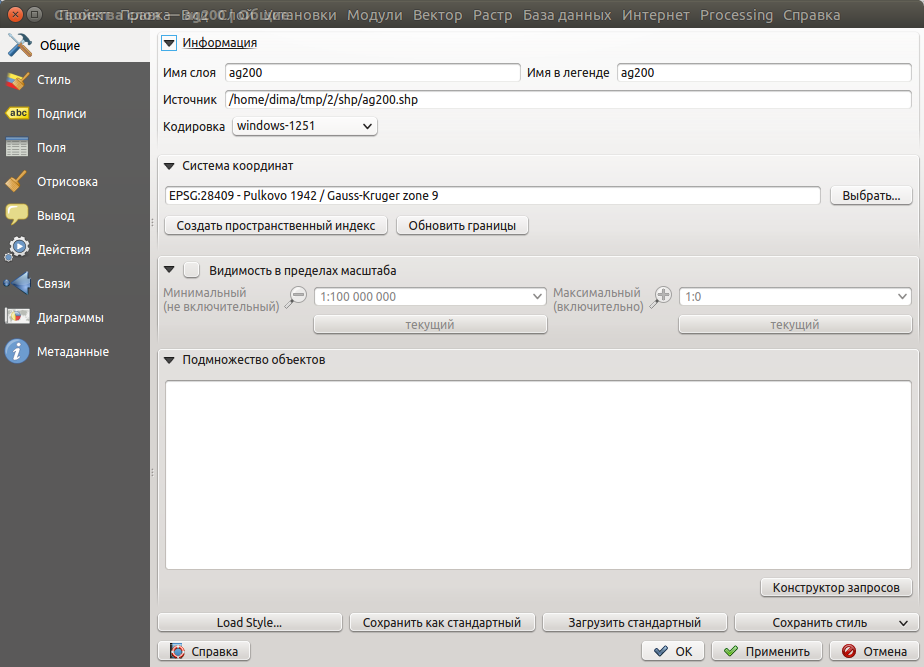
\includegraphics[width=0.95\columnwidth]{./practic/img/common.png}
           \end{center}
       \end{figure}
       Видимость в пределах масштаба.
\end{frame}

\begin{frame}
    \frametitle{Вкладка Стиль}
    \begin{figure}[!ht]
           \begin{center}
               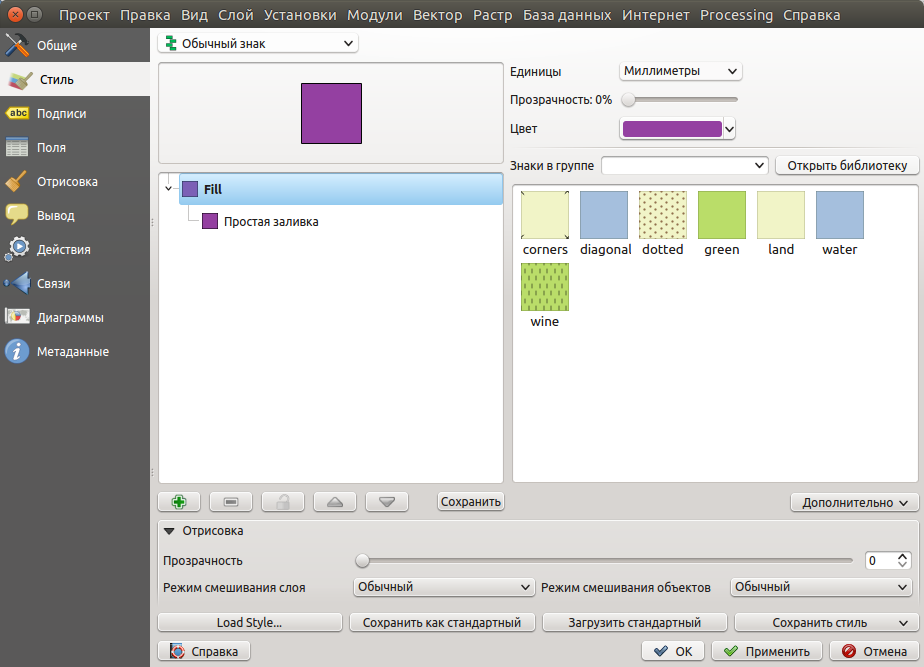
\includegraphics[width=0.95\columnwidth]{./practic/img/style.png}
           \end{center}
       \end{figure}
       Основная вкладка по стилям.
\end{frame}

\begin{frame}[allowframebreaks]
    \frametitle{Вкладка Стиль: градуировка знака}
    \begin{itemize}
        \item Обычный знак
        \item Уникальные значения (номинальные)
        \item Градуированный знак (порядковые)
        \item Правила (фильтр по значениям и видимость в пределах масштаба)
        \item Точки со смещением
        \item Инвертированные полигоны (фон -- цветом полигона, полигон -- белым)
    \end{itemize}
\end{frame}

\begin{frame}[allowframebreaks]
    \frametitle{Вкладка Стиль: режим смешения слоев}
    Пиксели, принадлежащие текущему слою и нижележащим слоям, смешиваются в соответствии с заданным алгоритмом.
    \begin{itemize}
        \item Normal: Цвета не смешиваются.
        \item Lighten: Выбирается самый светлый из всех нижележащих слоев.
        \item Screen: Светлые пиксели низлежащих слоев отрисовываются в текущем, а темные нет. (Используется для копирования текстур с других слоев).
        \item Dodge: Осветление низлежащих пикселей до уровня яркости пикселя текущего слоя.
        \item Addition: Суммирование яркостей пикселей слоев. Если сумма больше 1, получаем белый цвет.
        \item Darken: Выбирается самый темый пиксель.
        \item Multiply: Умножаются яркости пикселей.
        \item Burn: Темные пиксели верхнего слоя затемняют пиксели низлежащего слоя.
        \item Overlay: Комбинация Multiply и Screen.
        \item Soft light: Комбинация Burn и Dodge.
        \item Difference: Вычитается из вернего пикселя пиксель нижнего пиксель (или наоборот --- чтобы не уйти в минус).
        \item Subtract: Как и ранее, из верхнего вычитается минимум, но отрицательные значения заменяются нулем.
    \end{itemize}
\end{frame}

\begin{frame}
    \frametitle{Вкладка Подписи}
    \begin{figure}[!ht]
           \begin{center}
               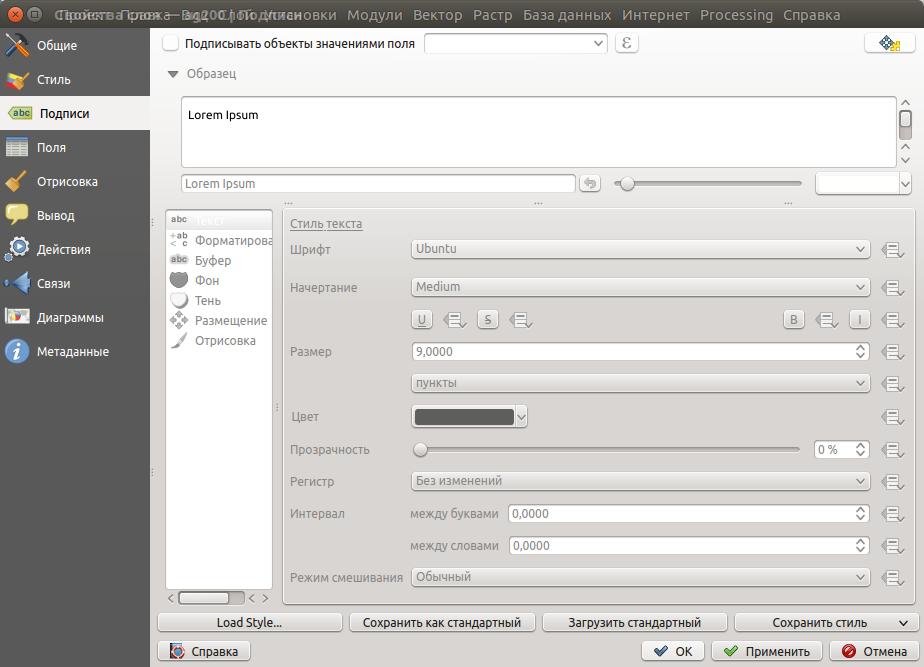
\includegraphics[width=0.95\columnwidth]{./practic/img/labels.png}
           \end{center}
       \end{figure}
\end{frame}

\begin{frame}
    \frametitle{Вкладка Вывод}
    \begin{figure}[!ht]
           \begin{center}
               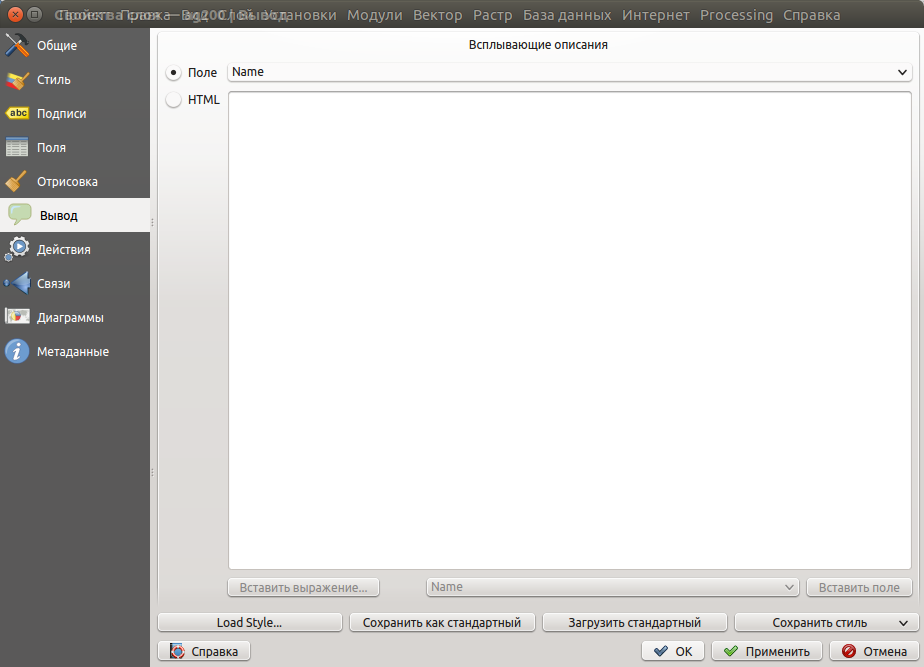
\includegraphics[width=0.95\columnwidth]{./practic/img/hints.png}
           \end{center}
       \end{figure}
\end{frame}


\begin{frame}
    \frametitle{Вкладка Диаграммы}
    \begin{figure}[!ht]
           \begin{center}
               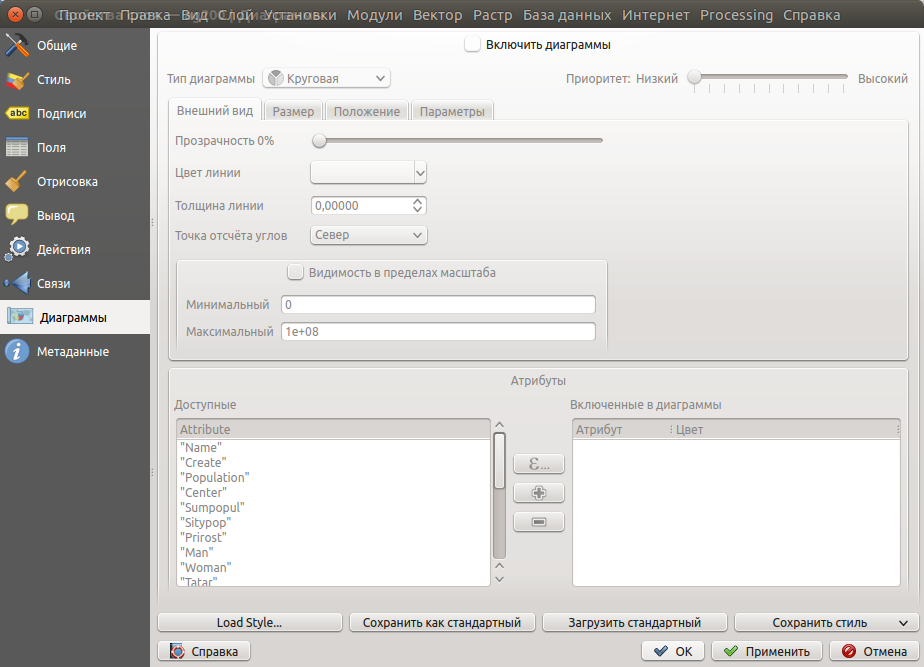
\includegraphics[width=0.95\columnwidth]{./practic/img/diagrams.png}
           \end{center}
       \end{figure}
\end{frame}

\begin{frame}
    \frametitle{Задание}
    Масштаб 1: в этом масштабе в окне видна вся карта. Видны общие границы республики и границы районов с названиями, административные центры в виде точки. На карту выводятся подписи районов.

    Масштаб 2: в этом масштабе в окне видна карта выбранного района с его названием. При достижении данного масштаба видны дороги и реки, административные центры нанесены на карту в виде точки.

    Масштаб 3: в этом масштабе ваш район достигает увеличения в 2 раза  (масштаб 3 крупнее масштаба 2 в 2 раза), при этом должны быть видны все слои, а также отображаться названия населенных пунктов. Административный центр не должен отображаться точкой.

    Масштаб 4: в этом масштабе района достигает увеличения в 4 раза. В этом масштабе на карте видны все слои, названия населенных пунктов и рек. Название района не отображается.

    Масштаб 5: в этом масштабе карта района достигает увеличения в 8 раз. Видны все слои и названия всех объектов.
\end{frame}


\begin{frame}
    \frametitle{Кодировка типов автодорог}
    \begin{description}
        \item[61210000] Автомагистрали (автострады)
        \item[61220000] Автодороги с улучшенным покрытием
        \item[61230000] Автодороги с покрытием (шоссе)
        \item[61240000] Дороги с твердым покрытием
        \item[61310000] Автодороги без покрытия
        \item[61320000] Грунтовые проселочные дороги
        \item[61330000] Полевые и лесные дороги
        \item[61500000] Автодороги с дерев. покрытием
        \item[61940000] Труднопроезжие участки дорог
    \end{description}
\end{frame}


    %~ \subsection{Инструменты ftools}
    %~ 
\begin{frame}
    \frametitle{Задания}
    \begin{itemize}
        \item Построить картографический слой населенных пунктов Татарстана, расположенных на расстоянии не более 15 км от райцентров.
        \item Построить картографический слой населенных пунктов, целиком входящих в границы заданного района, расположенных на расстоянии более 5 км от автострады (от шоссейных дорог вашего района).
        \item Найти длины дорог, лежащих внутри районов. % Сама задача простая, но часть полигонов некорректна. Нужно их найти и исправить проблему. Только потом можно считать.
        \item Рассчитать длину дорог с улучшенным покрытием внутри районов.
        \item Найти переправы через реки в Азнакаевском районе.
    \end{itemize}
\end{frame}

%~
    %~ \subsection{DBMamager}
    %~ 
\begin{frame}[allowframebreaks]
    \frametitle{Задачи}
    \begin{itemize}
        \item Создать выборку районов где численность городского населения превышает сельское (разница населения)
        \item Создать слой населенных пунктов принадлежащих районам из предыдущего задания (связь по полям Tanp.Agnum=ag200.Kodname)
        \item Создать слой населенных пунктов принадлежащих районам из предыдущего задания (связь по геометрии)
        \item Определить численность населения в районах созданных в 1930,1938,1965 годах.
        \item Построить запрос для отображения района с минимальным приростом. Использовать слой Ag200.
        \item Построить картографический слой административных районов РТ, пересекаемых хотя бы одной улучшенной шоссейной дорогой.
        \item Построить картографический слой административных районов РТ, пересекаемых ровно четырьмя шоссейными дорогами.
        \item Построить картографический слой улучшенных шоссейных дорог, целиком находящихся внутри одного административного района РТ.
        \item Выбрать все дороги, которые пересекаются (граничат) с aдминистративным центором. (Административные центры хранятся в точечном слое taadmp, поэтому для поиска полигональных административных центров нужно предварительно выбрать объекты из слоя Tanp).
        \item Построить последовательность запросов для поиска населенных пунктов (картографический слой Tanp), расположенных на расстоянии не более 10 км от шоссейных дорог в тех административных районах, плотность населения которых выше средней по республике.
    \end{itemize}
\end{frame}

\begin{frame}
    \frametitle{Упрощение геометрии}
    CREATE VIEW simpl AS SELECT pk, name, Simplify(geom, 200) FROM ag200 WHERE name='Верхнеуслонский'
\end{frame}


    \subsection{Построение зон доступности с использованием инструментов GRASS}
    
\begin{frame}
    \frametitle{Построение зон доступности с использованием GRASS}
    \begin{block}{Задача}
        Имеется информация о точках и маршрутах движения. Требуется построить зоны доступности от каждой точки, например,
        зоны пешеходной доступности в 200, 400, 600, \dots метров.

        Ограничения: пространство считается неоднородным с точки зрения движения. Например, пешеход пойдет скорее по дорогам, чем
        по бездорожью; существуют участки, которые недоступны для прохода (здания, промзоны и т.п.).
    \end{block}

\end{frame}

\begin{frame}
    \frametitle{Построение зон доступности с использованием GRASS}
    Задача может быть решена с двух разных подходов:
    \begin{itemize}
        \item Векторный подход (построение графа дорог и поиск пути по этому графу):
        \begin{itemize}
            \item преимущество подхода: точность расчетов движения по дорогам;
            \item недостатки подхода: невозможно построить маршрут через области, в которых не проходит дорога (в реальной жизни пешеход может срезать углы).
        \end{itemize}
        \item Растровый подход (построение растра стоимости движения и расчет суммарной стоимости движения от точек):
        \begin{itemize}
            \item преимущество подхода: при создании растра стоимости движения мы не ограничены местоположениями дорог и можем строить пути в произвольных областях;
            \item недостатки подхода: при создании растра стоимости нужно назначить цену движения через ячейку растра; выбор объективной стоимости может оказаться достаточно сложной задачей.
        \end{itemize}
    \end{itemize}
\end{frame}

\begin{frame}
    \frametitle{Пример данных}
    \begin{figure}[!ht]
        \begin{center}
            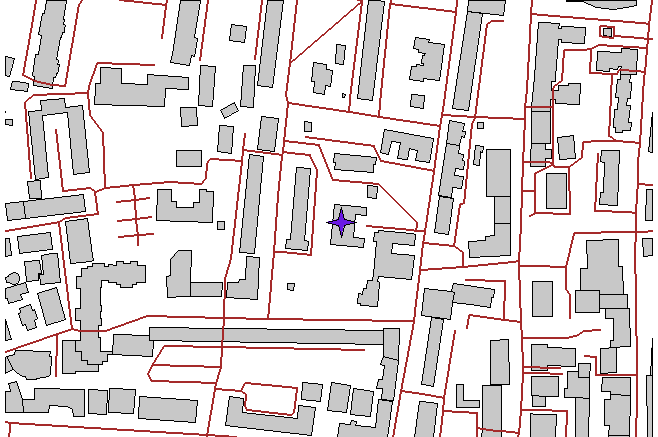
\includegraphics[width=0.6\columnwidth]{./practic/img/area_of_interest.png}
        \end{center}
    \end{figure}
    На карте представлены:
    \begin{itemize}
        \item Здания (buildings): серые многоугольники
        \item Дороги (roads): красные линии
        \item Объект, тоступность которого измеряется обозначен синей звездой (mypoint).
    \end{itemize}

\end{frame}

\begin{frame}
    \frametitle{Решение на базе векторного подхода: идея}
    Общий план действий:
    \begin{enumerate}
        \item Строим топологически корректный граф дорог и присоединяем к нему точку, для которой будем оценивать зоны доступности.
        \item Делим полученный граф дорог на зоны доступности.
    \end{enumerate}
\end{frame}

\begin{frame}[allowframebreaks,fragile]
    \frametitle{Решение на базе векторного подхода: реализация}
    \begin{enumerate}
        \item Строим топологически корректный граф дорог и присоединяем к нему точку, для которой будем оценивать зоны доступности:
        \begin{enumerate}
            \item В ходе векторизации дороги могли быть построены так, что они пересекаются визуально, но общей вершины у них нет. Воспользуемся инструментом v.clean, чтобы добавить общие вершины:
            \begin{verbatim}
v.clean in=roads out=roads_br
    tool=snap,break,rmdupl thre=0.5,0,0
            \end{verbatim}
            здесь мы <<прищелкнули>> вершины друг к другу, если они лежат ближе, чем 0.5 метра, затем разбили линии в точках пересечения (добавили к ним вершины) и удалили возможные дубликаты линий. В результате был получен новый векторный слой roads\_br.
            \item Создадим граф дорог (roads\_network), добавив к нему точки из слоя mypoint (присоединим точки, если они лежат на расстоянии от дорог меньшем, чем 10 километров):
            \begin{verbatim}
v.net input=roads_br points=mypoint
    output=road_network
    operation=connect thresh=10000
            \end{verbatim}
            Результат показан на рисунке (заметим на будущее, что точка была присоеденена к дороге, проходящей к востоку от нее):
            \begin{figure}[!ht]
                \begin{center}
                    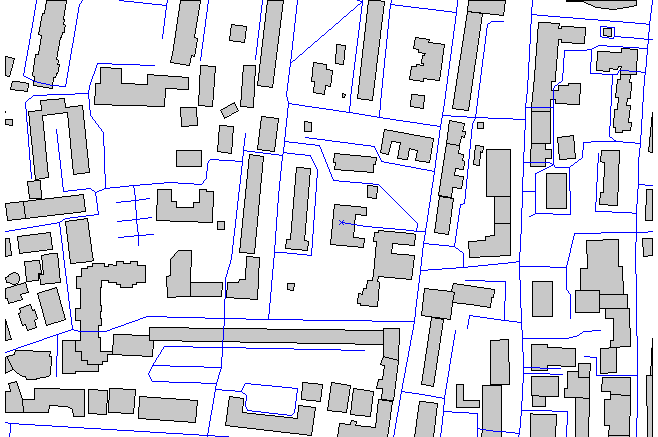
\includegraphics[width=0.8\columnwidth]{./practic/img/roads_network}
                \end{center}
            \end{figure}
        \end{enumerate}
        \item Делим полученный граф дорог на зоны доступности, которые будем рассчитывать для точек с категориями от 1 до 1000000 (здесь берем категории с запасом; можно указать категории конкретных точек) слоя road\_network:
        \begin{verbatim}
v.net.iso input=road_network
    output=road_network_iso
    ccats=1-1000000 costs=250
            \end{verbatim}
    \end{enumerate}
    Построенный граф road\_network\_iso содержит два типа линий: категория 1 -- линии, которые лежат ближе, чем 250 метров и категория 2 --- линии, которые лежат далее, чем 250 метров (можно было разбить граф на большее число категорий). Результат показан на рисунке:
            \begin{figure}[!ht]
                \begin{center}
                    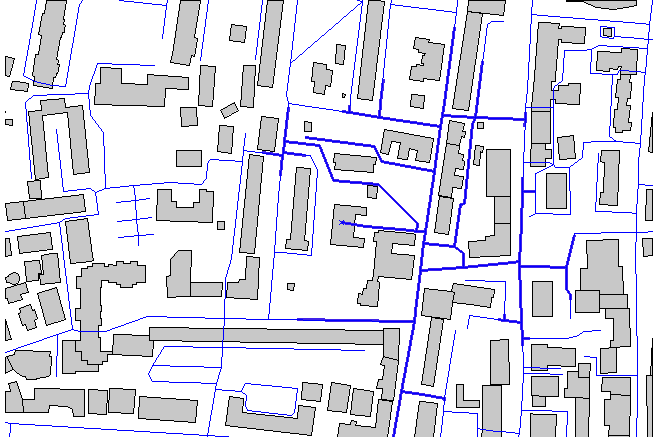
\includegraphics[width=0.9\columnwidth]{./practic/img/roads_iso}
                \end{center}
                \caption{Зоны доступности}
            \end{figure}
    Как видим, зона доступности к западу от точки значительно меньше, чем к востоку (вспомним, что точка была присоеденена к дороге, проходящей к востоку от нее), хотя расстояние от точки до ближайшей западной дороги было лишь незначительно больше, чем до ближайшей восточной.
\end{frame}

\begin{frame}
    \frametitle{Замечания}
    \begin{itemize}
        \item Мы строили граф дорог и расчитывали по нему расстояния, используя в качестве веса ребра графа его длину в географическом пространстве. GRASS позволяет использовать таблицу аттрибутов для назначения веса ребрам графа.
        \item Мы считали, что движение по дорогам может идти в обоих направлениях. При необходимости можно указать что ребра графа являются однонаправленными.
    \end{itemize}
    Более подробную информацию об этих и других параметрах модулей см. в документации.
\end{frame}


\begin{frame}
    \frametitle{Решение на базе растрового подхода: идея}
    Общий план действий:
    \begin{enumerate}
        \item Построим растр стоимости движения, который будет показывать, насколько сложно пройти через ячейку: если ячейка принадлежит зданию, цена прохода будет очень большой, если же проход через ячейку свободен, то назначим цену прохода через нее равным ширине (высоте) ячейки.
        \item Запустим процедуру поиска доступности заданной точки, используя растр стоимости. В результате будет найден растр суммарной цены прохода: в ячеке растра будет храниться цена передвижения от ячейки до точки.
        \item (Опционально) Построим полигоны, соответствующие зонам доступности.
    \end{enumerate}
\end{frame}

\begin{frame}[fragile,allowframebreaks]
    \frametitle{Решение на базе растрового подхода: реализация}
    \begin{enumerate}
        \item Построение растра стоимости.
        \begin{enumerate}
            \item Зададим размер ячейки растра равным одному метру:
            \begin{verbatim}
g.region res=1 -p
            \end{verbatim}
            \item Растеризуем здания, указав, что ячейки, лежащие под зданиями должны иметь большое значение (10000):
            \begin{verbatim}
v.to.rast in=buildings_aoi
    out=buildings_aoi use=val val=10000
            \end{verbatim}
            \item Построим растр стоимости:
            \begin{verbatim}
r.mapcalc "cost=1"
r.mapcalc "cost=
    if(isnull(buildings_aoi),
        cost, buildings_aoi)"
            \end{verbatim}
            \item Растеризуем точки (точка может попасть на здание, как и в нашем случае, поэтому увеличим ее размер, чтобы она вышла за пределы здания):
            \begin{verbatim}
v.to.rast mypoint out=mypoint use=val val=1
r.grow mypoint out=point radius=10
            \end{verbatim}
            \item Впечатаем точку в растр стоимости, чтобы она <<прорезала>> здание:
            \begin{verbatim}
r.mapcalc "cost=if(isnull(point), cost, point)"
            \end{verbatim}
            Растр стоимости показан на рисунке:
            \begin{figure}[!ht]
                \begin{center}
                    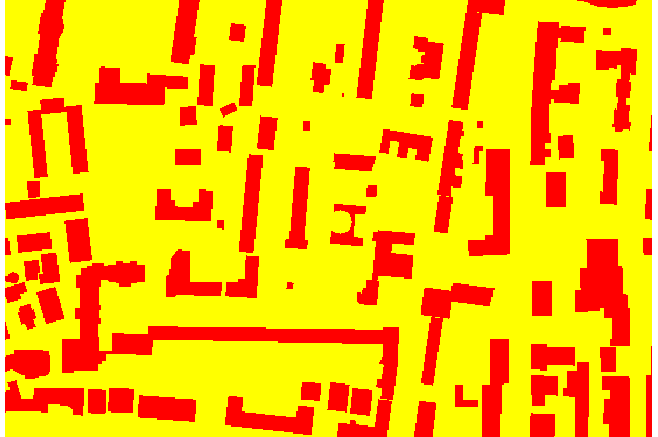
\includegraphics[width=0.8\columnwidth]{./practic/img/cost}
                \end{center}
                \caption{Стоимость движения через ячейки (красный цвет --- 10000, желтый --- 1)}
            \end{figure}
        \end{enumerate}
        \item Зоны доступности:
        \begin{enumerate}
            \item Построим растр суммарной стоимости движения
            \begin{verbatim}
r.cost -k in=cost output=distance
    start_point=mypoint max_cost=250
r.mapcalc "distance =
    if(distance<=250, distance, null())"
            \end{verbatim}
            В последней команде мы удаляем из растра все ячейки, стомость пути до которых превышает 250.
            \begin{figure}[!ht]
                \begin{center}
                    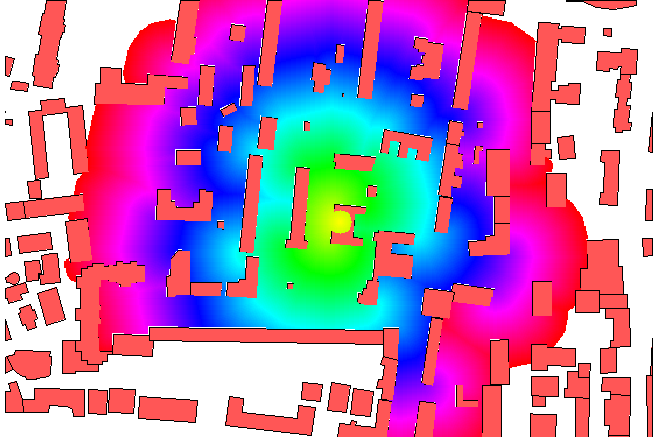
\includegraphics[width=0.8\columnwidth]{./practic/img/cum_cost}
                \end{center}
                \caption{Суммарная стоимость движения от точки mypoint}
            \end{figure}
            \item Построим векторные изолинии стоимости движения шагом 50 метров:
            \begin{verbatim}
r.mapcalc "iso_dist = 50 *int(distance/50)"
r.to.vect in=iso_dist out=distance feature=area
            \end{verbatim}
            Результат показан на рисунке:
            \begin{figure}[!ht]
                \begin{center}
                    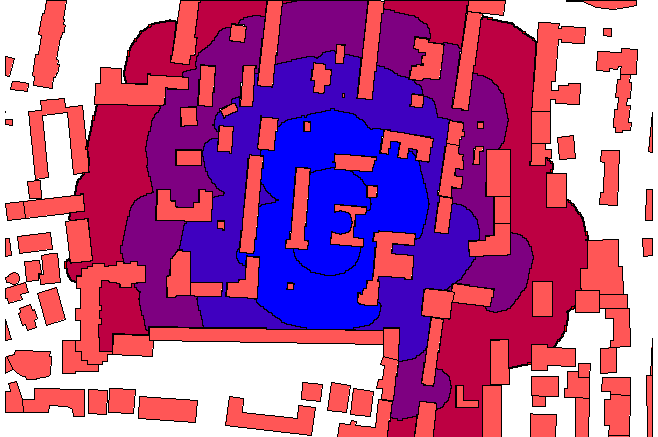
\includegraphics[width=0.8\columnwidth]{./practic/img/vector_cum_cost}
                \end{center}
                \caption{Изолинии стоимости движения от точки mypoint}
            \end{figure}
        \end{enumerate}
    \end{enumerate}
\end{frame}

\begin{frame}[fragile,allowframebreaks]
    \frametitle{Дополнительный пример}
    В предыдущем примере стоимость движения была одинакова во всех направлениях, наличие дорог не учитывалось. Можно учесть, что
    по дороге идти легче (допустим в два раза), тогда:
    \begin{verbatim}
g.region res=1 -p
v.to.rast in=buildings_aoi
    out=buildings_aoi use=val val=10000
v.to.rast roads out=roads use=val val=1

r.mapcalc "cost=2"  # пустое место
r.mapcalc "cost=
    if(isnull(buildings_aoi), cost, buildings_aoi)"
r.mapcalc "cost=
    if(isnull(roads), cost, roads)"

v.to.rast mypoint out=mypoint use=val val=1
r.grow mypoint out=point radius=10
r.mapcalc "cost=if(isnull(point), cost, point)"

r.cost -k in=cost output=distance
    start_point=mypoint max_cost=250
r.mapcalc "distance =
    if(distance<=250, distance, null())"
    \end{verbatim}
    \begin{figure}[!ht]
        \begin{center}
            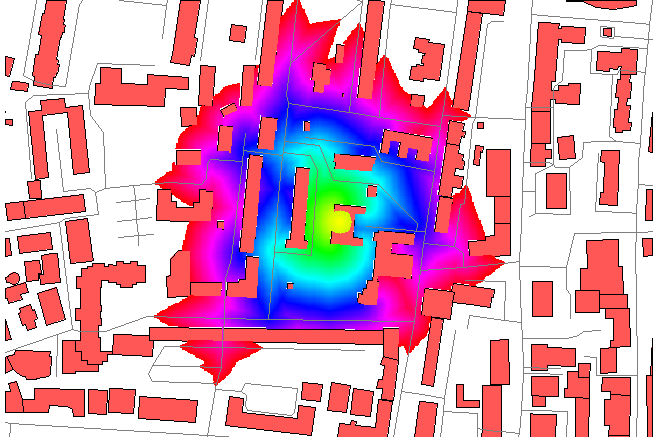
\includegraphics[width=0.9\columnwidth]{./practic/img/cum_cost2}
        \end{center}
        \caption{Суммарная стоимость движения от точки mypoint с учетом дорог}
    \end{figure}
\end{frame}




\mode*

\end{document}

